\documentclass[12pt,a4paper]{article}
\usepackage[utf8]{inputenc}
\usepackage[german]{babel}
\usepackage[T1]{fontenc}
\usepackage{amsmath}
\usepackage{amsfonts}
\usepackage{amssymb}
\usepackage{hyperref}
\usepackage{listings}
\usepackage{color}
\usepackage{graphicx}
\usepackage[section]{placeins}
\usepackage{comment}
\author{Jonathan Weißenberger}
\title{Semesterarbeit OpenPEARL}

\definecolor{dkgreen}{rgb}{0,0.6,0}
\definecolor{gray}{rgb}{0.5,0.5,0.5}
\definecolor{mauve}{rgb}{0.58,0,0.82}

\begin{comment}
\lstset{
frame=single, breaklines=true,
postbreak=\raisebox{0ex}[0ex][0ex]{\ensuremath{\color{red}\hookrightarrow\space}}, numbers=left, numbersep=5pt
}
\end{comment}

\lstset{frame=tb,
  language=Java,
  aboveskip=3mm,
  belowskip=3mm,
  showstringspaces=false,
  columns=flexible,
  basicstyle={\small\ttfamily},
  numbers=none,
  numberstyle=\tiny\color{gray},
  keywordstyle=\color{blue},
  commentstyle=\color{dkgreen},
  stringstyle=\color{black},
  breaklines=true,
  breakatwhitespace=true,
  tabsize=3
}
\begin{document}
\maketitle
\newpage
\tableofcontents
\newpage
\listoffigures
\newpage
\section[(Jonathan Weißenberger) Allgemeine Beschreibung]{Jonathan Weißenberger\\Allgemeine Beschreibung}
Das Team, bestehend aus Alexander Hebel, Dennis Seilnacht und Jonathan Weißenberger beschäftigen sich im vierten Semester mit der Portierung der Umgebung OpenPEARL für Microcontroller. Das Target in der Portierung ist das Entwicklungsboard STM32F746-DISCO. Zusätzlich zur Portierung erfolgt eine Demoapplikation. Hierbei ist die bereits existierende Kugelsortierungsanlage der Hochschule Furtwangen mit dem Microcontrollerboard zu steuern.
\begin{figure}[h]
\begin{center}
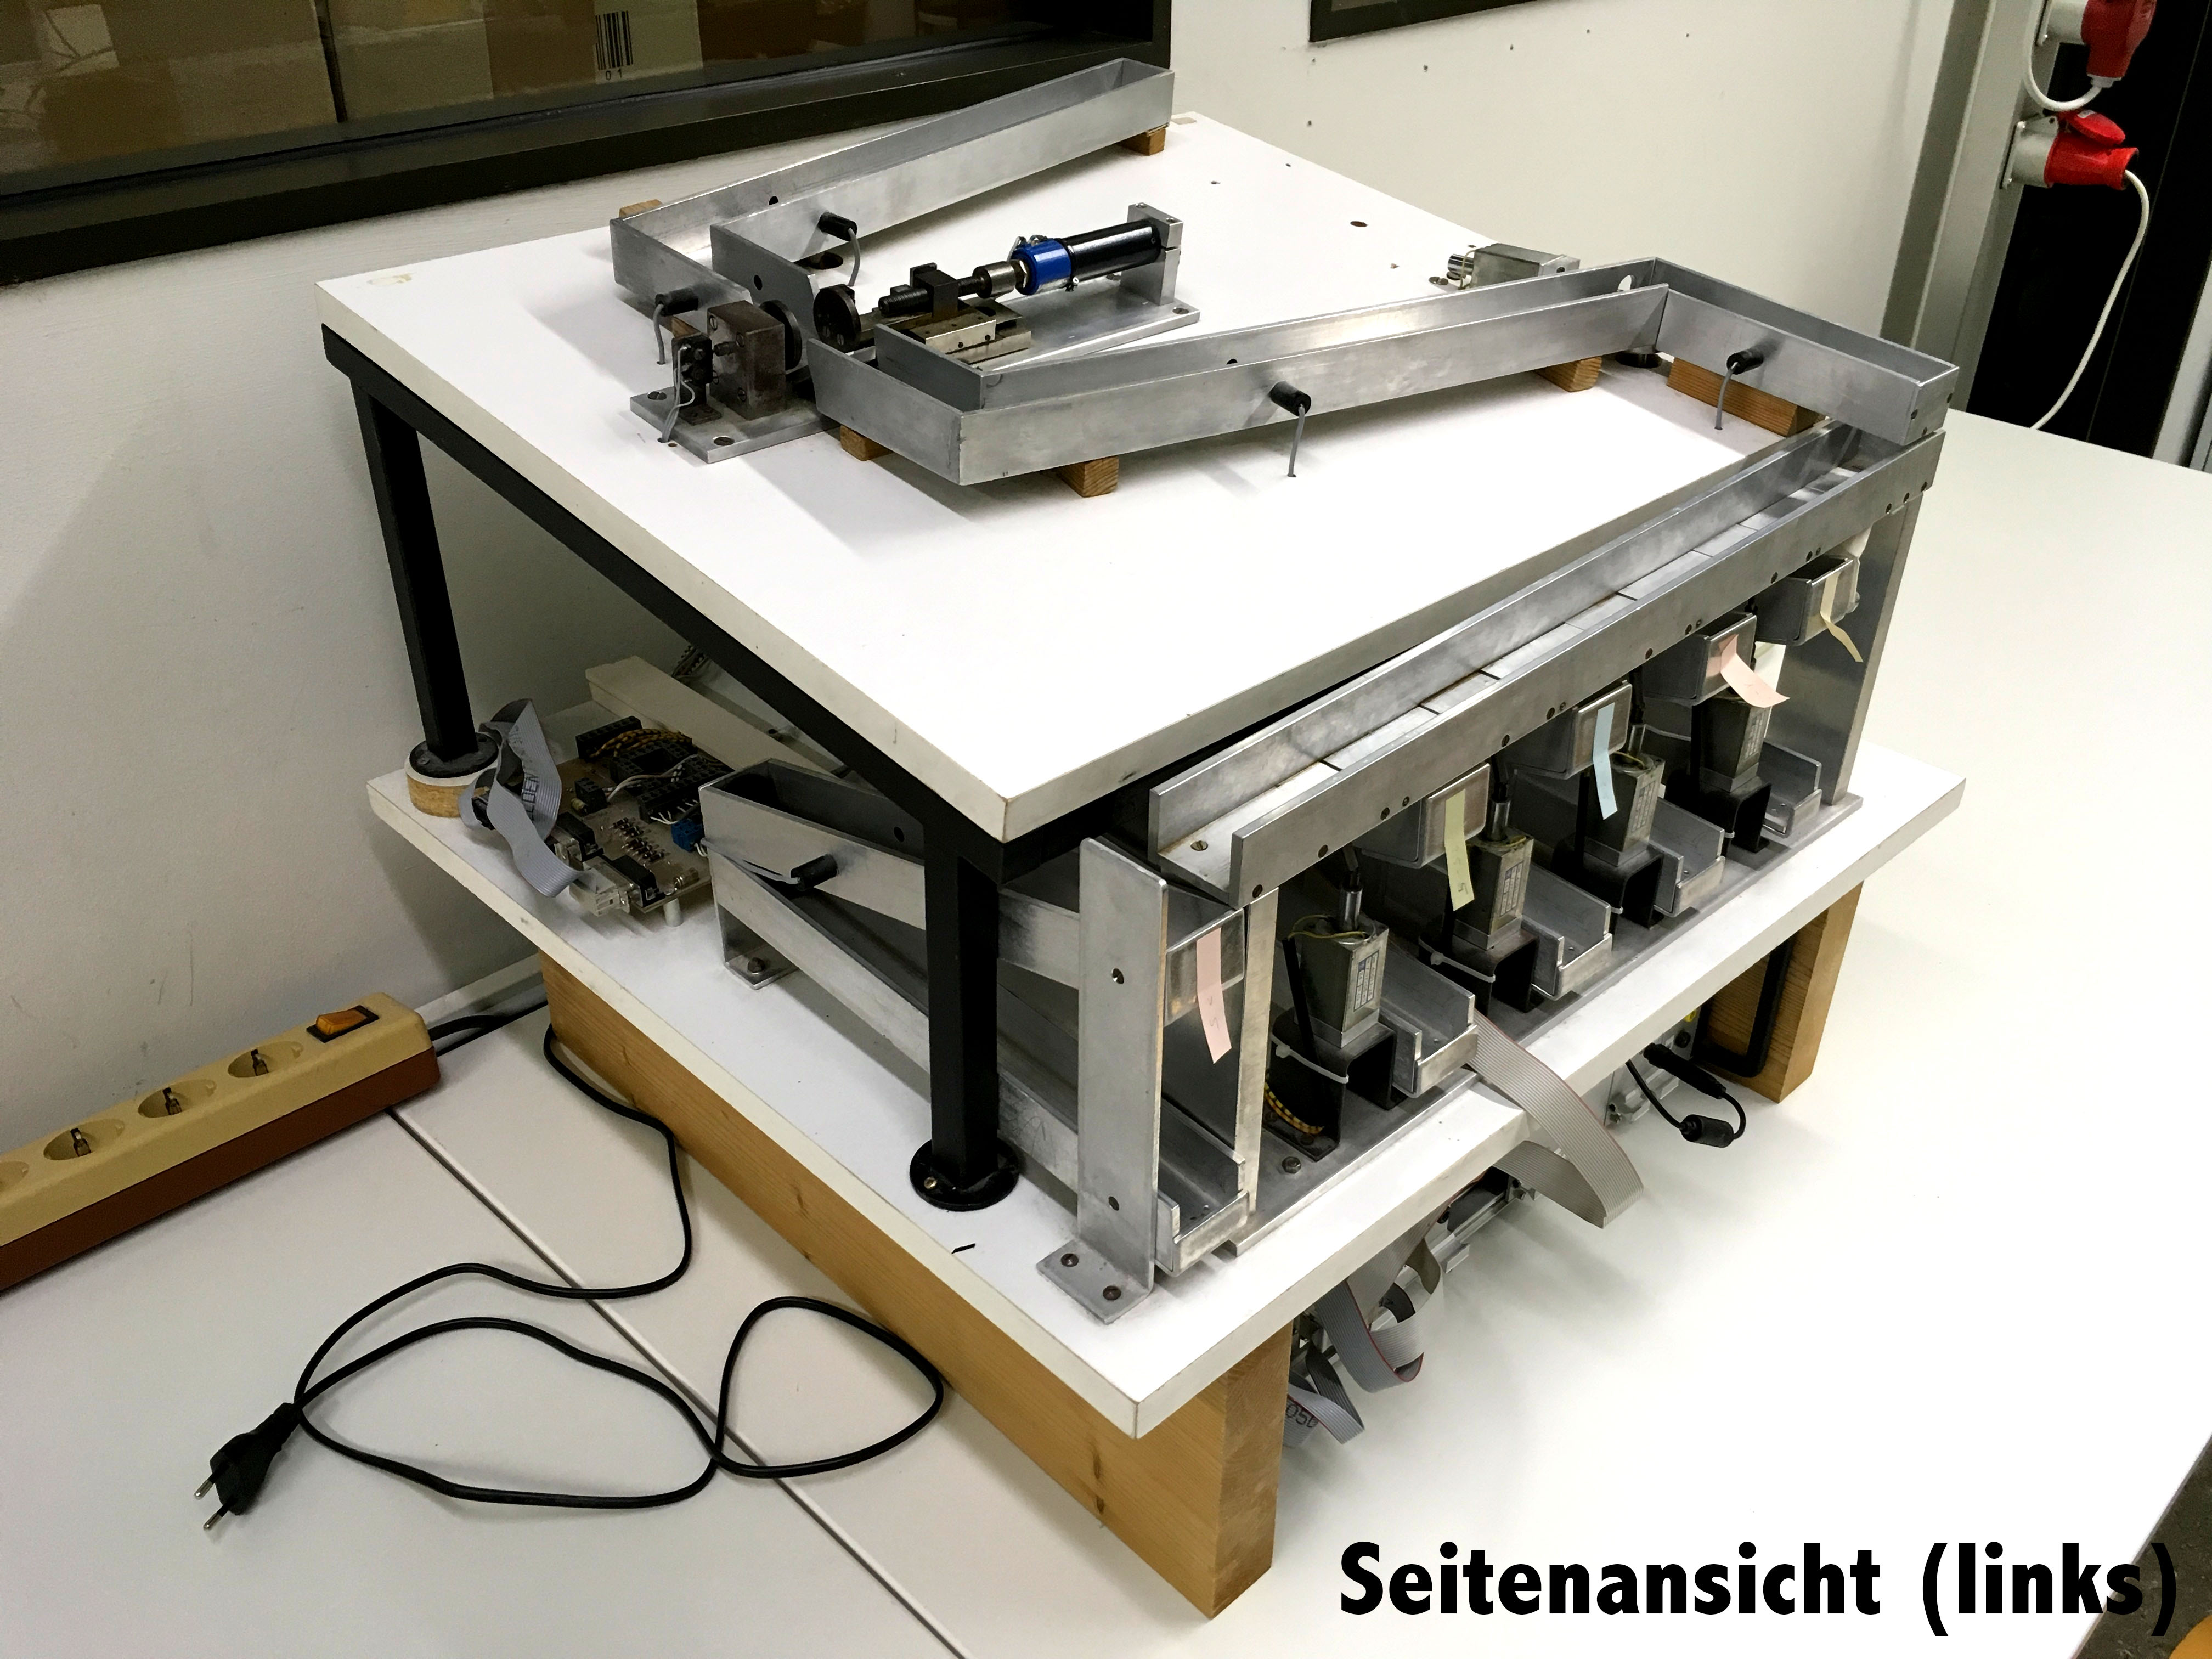
\includegraphics[width=10cm]{grafiken/Seitenansicht.jpg}
\label{bild_kugelsortiermaschine}
\caption{Kugelsortiermaschine}
\end{center}
\end{figure}
Das primäre Ziel der Arbeit ist die Lauffähigkeit von OpenPEARL auf der Zielplattform. Im Konkreten bedeutet das, dass Software in der Sprache OpenPEARL übersetzt werden kann und dann nach der Übertragung auf dem Zielsystem läuft. Das Kompilat soll nachvollziehbare Ergebnisse liefern, die wir zuvor definieren. Im Fall der Sortierungsanlage sollen die Kugeln ihrer jeweiligen Dichte entsprechend in die einzelnen Fächer eingeordnet werden. Die Dichte errechnet sich dann aus dem Durchmesser der Kugel und dem Gewicht ($Dichte=Masse/Volumen$). Zu den Funktionalitäten, die mit OpenPEARL genutzt werden sollen gehört das $I^2C$-Bussystem. Durch das Bussystem wird die Kugelsortierungsmaschine angesteuert und Informationen abgerufen. Außerdem soll eine Kommunikationsverbindung mit dem Target mittels UART-Schnittstelle von einem Host-Computer aus möglich sein. Durch die Schnittstelle soll es möglich sein, Befehle an den Microcontroller zu senden und Informationen abzurufen. 
\begin{figure}[h]
\begin{center}
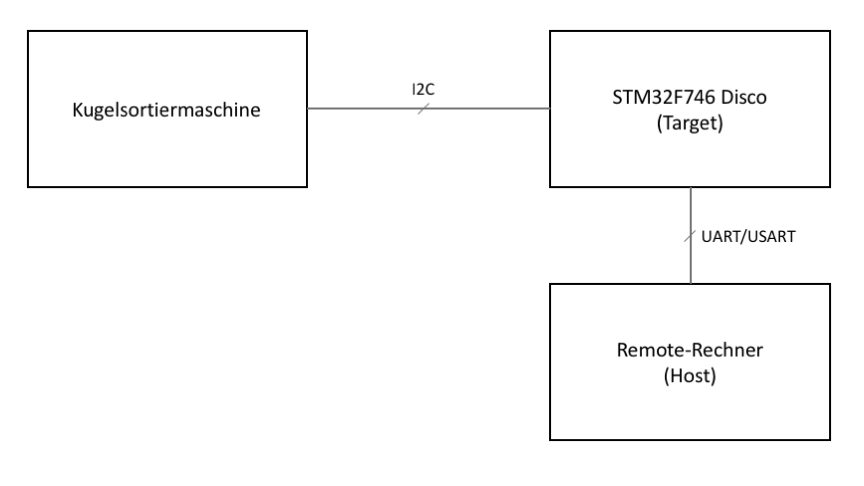
\includegraphics[width=10cm]{grafiken/Schematik.png}
\caption{Schematik des Projektaufbaus}
\label{schematik_projektaufbau}
\end{center}
\end{figure}
Sofern die Grundfunktionalitäten in angemessener Zeit umgesetzt werden können, wird zusätzlich die Verwendbarkeit des Displays angestrebt. Das Display soll zusätzlich Statusberichte liefern über den Zustand der Sortierungsanlage. 
\subsection{Beschreibung der Kugelsortiermaschine}
Die Sortiermaschine wird von der Hochschule Furtwangen bereitgestellt. In diesem Abschnitt wird im Wesentlichen die Funktionalität und die Bestandteile der Sortiermaschine geklärt.
Der Einwurf der Kugeln erfolgt von Hand. In der Draufsicht (siehe Abbildung), ist die Laufbahn, die Ballführung zu erkennen. Dadurch, dass die Führung leicht abschüssig ist, rollen die Kugeln. Auf dem Weg nach unten, passieren die Kugeln mehrere Lichtschranken. Durch diese Lichtschranken ist es möglich, die Schienen in Abschnitte einzuteilen und mehrere Kugeln gleichzeitig erfassen zu können. Wenn beispielsweise eine Kugel Lichtschranke 3 passiert, kann im Balleinwurf schon eine neue Kugel eingegeben werden. Die Durchmesserbestimmung ist im wesentlichen ein Motor, der eine Gewindestange in Richtung Rollbahn bewegt. Nachdem eine Kugel eingeworfen wurde, rollt diese als erstes in Richtung dieser Messeinheit. Durch eine Klappe von unten wird die Kugel an der Messstation gestoppt. Wie bereits beschrieben, wird die Gewindestange dann in Richtung Rollfeld gedreht, bis ein Taster ausgelöst wird. Anschließend wird der Potentiometerwert ausgelesen. Bei dem Potentiometer handelt es sich um einen Drehpotentiometer, dessen Widerstandswert sich mit dem Drehen der Gewindestange verändert. Anhand dieses Wertes kann der Durchmesser der Kugel bestimmt werden. Ist der Wert gelesen, wird die Gewindestange zurückgefahren und die Bodenklappe lässt den Ball weiterrollen. Die nächste Station, die von der Kugel passiert wird ist die Waageeinheit. Sie ermittelt das Gewicht der Kugel. Durch eine Kule auf der Waagefläche bleibt die Kugel auf der Waage liegen. Sobald der Wert gelesen ist, wird die Kugel durch einen Bolzen herausgeschossen. Anhand der ermittelten Dichte wird dann bestimmt, welche Klappe sich öffnet. Die jeweilige Klappe bestimmt darüber, in welchem Fach die Kugel landet.
\begin{figure}[h]
\begin{center}
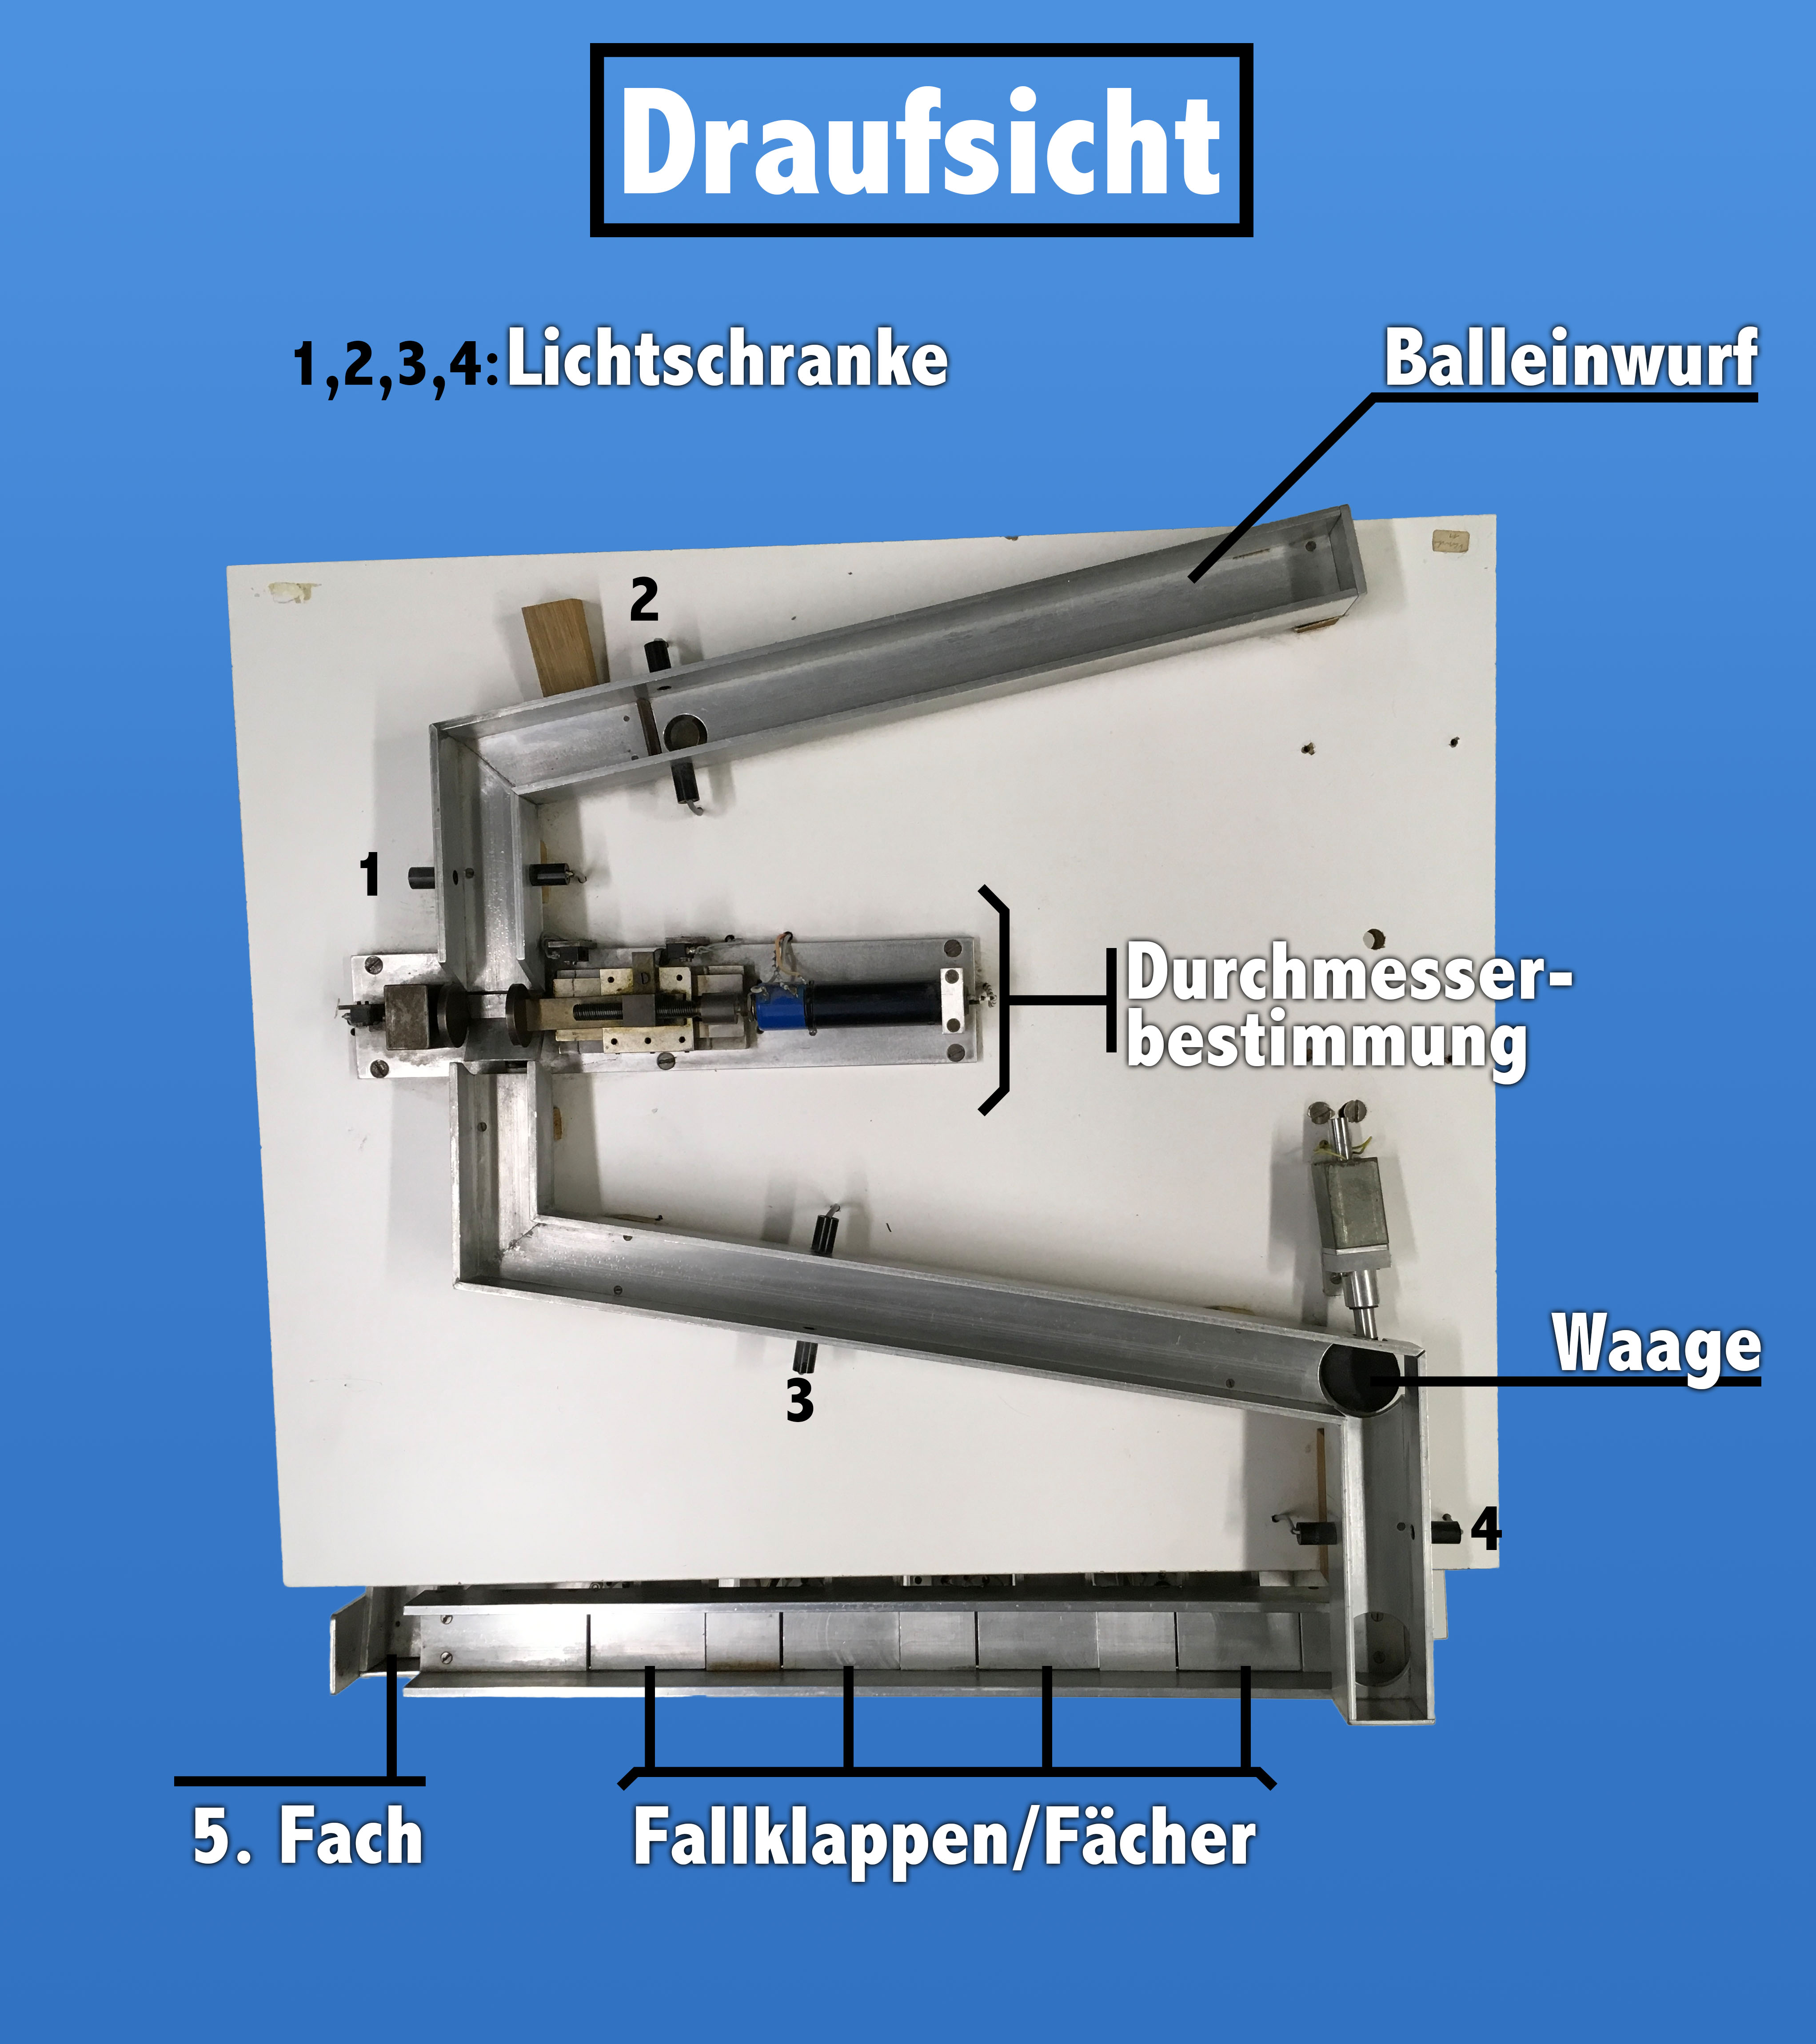
\includegraphics[width=12cm]{grafiken/Draufsicht.jpg}
\caption{Die Draufsicht auf die Demoapparatur}
\label{draufsicht_sortiermaschine}
\end{center}
\end{figure}

\subsection{Beschreibung des Zeitplans}
Der ausgearbeitete Zeitplan war erst erstellbar nach den ersten Wochen. Nach diesem Zeitraum waren schon Toolchain, Debuggerinstallation und Testprogrammausführung vollendet. 
\begin{figure}[h]
\begin{center}
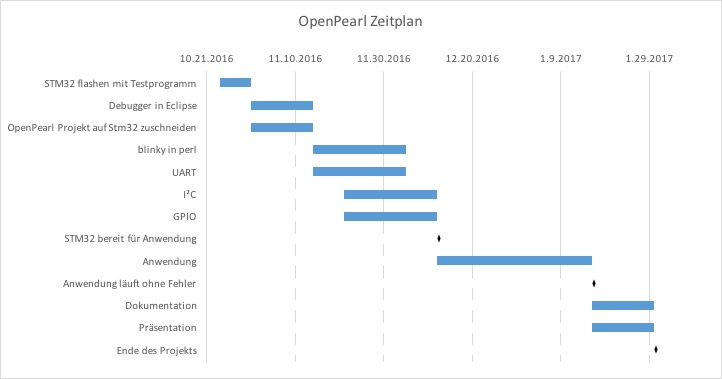
\includegraphics[width=13.5cm]{grafiken/zeitplan.jpg}
\caption{Zeitplan als Ergebnis des Meetings am 09.11.2016}
\label{zeitplan}
\end{center}
\end{figure}

\subsection{Anwendungsbeschreibung}
Zum Ende des Semesters soll eine Steuerung der oben beschriebenen Kugelsortiermaschine möglich und die Funktionen, die im Abschnitt 'Beschreibung der Kugelsortiermaschine' beschrieben sind steuerbar sein. Zum Einsatz kommt der I2C-Bus. Durch Adressierung der unterschiedlichen Gerätschaften in der Kugelsortiermaschine wird die Steuerung gewährleistet. Adressierbar sind Lichtschranken, Waage, Motor, Klappen und Stoßer.
\newpage
\chapter{Einrichtung des Debuggers}
In diesem Kapitel wird im Stil eines Tutorials vorgestellt, wie wir vorgegangen sind, um den Debugger zum Laufen zu bekommen. Als Betriebssystem kam Debian zum Einsatz.
\section{st-flash Installation und UDEV-Rules}
st-flash wurde von uns anfangs benutzt, um die erzeugten Kompilate auf die Zielplattform zu überführen. In der Installationsroutine ist auch die Installation der wichtigen UDEV-Rules enthalten. Diese werden später noch benötigt.
Zuallererst muss das git-Repository heruntergeladen werden. Zusätzlich, falls nicht vorhanden noch ein paar nötige Build-Tools.
\begin{lstlisting}[language=sh]
sudo apt-get install cmake
sudo apt-get install libusb-1.0-0-dev git
git clone https://github.com/texane/stlink stlink.git
cd stlink.git
\end{lstlisting}
Sobald das Repository heruntergeladen ist, wechseln wir in das Projektverzeichnis und führen die Installationsprozedur aus. Zuerst das "make" und danach werden die ausführbaren Binarys in das "/usr/bin"-Verzeichnis kopiert.
\begin{lstlisting}[language=sh]
make
sudo cp build/Release/st-* /usr/bin
exit # -> Bash neu starten
\end{lstlisting}
Zum Schluss werden die udev-Rules gesetzt, damit das Gerät -also das Target- richtig erkannt wird.
\begin{lstlisting}
cd ~/stlink.git
ls -LR | grep rule
cd etc/udev/rules.d
sudo cp *.rules /etc/udev/rules.d
sudo udevadm --reload
sudo udevadm trigger
\end{lstlisting}
\section{Download Eclipse}
Um den Debugger zum Laufen zu bekommen, benötigt man zuallererst eine funktionierende Eclipse IDE. Für unser Projekt haben wir uns für 'Eclipse IDE for C/C++ Developers' entschieden erhältlich auf \url{http://www.eclipse.org/downloads/}.
Nach dem Download muss das Paket entpackt werden. In der Kommandozeile funktioniert dies mit dem Befehls 
\begin{lstlisting} 
tar -xzf <eclipse-download-file>
\end{lstlisting}
oder ganz einfach in der grafischen Benutzeroberfläche des Betriebssystems.
Um die Entwicklungsumgebung ausführen zu können, benötigt man Java-Version 1.8 der neuer. 
Die Installation hierfür funktioniert mit den folgenden Commands:
\begin{lstlisting}
sudo su -
echo "deb http://ppa.launchpad.net/webupd8team/java/ubuntu xenial main" | tee /etc/apt/sources.list.d/webupd 8team-java.list
echo "deb-src http://ppa.launchpad.net/webupd8team/java/ubuntu xenial main" | tee -a /etc/apt/sources.list.d/webupd8team-java.list
apt-key adv --keyserver hkp://keyserver.ubuntu.com:80 --recv-keys EEA14886
apt-get update
apt-get install oracle-java8-installer
apt-get install oracle-java8-set-default
exit

\end{lstlisting}
\section{Toolchain-Installation}
Um später debuggen zu können, wird ein Kompiler für die Zielplattform benötigt und der spezifische GDB. Diese Tools findet man in Toolchains. Eine Toolchain ist eine komplette Suite, mit Werkzeugen, um für fremde Hardwarearchitekturen Software bauen zu können.
Wir verwenden die GNU-Toolchain. Zunächst laden wir die komplette Toolchain herunter.
\begin{lstlisting}[language=sh]
cd /opt
sudo wget https://launchpad.net/gcc-arm-embedded/5.0/5-2016-q3-update/+download/gcc-arm-none-eabi-5_4-2016q3-20160926-linux.tar.bz2
\end{lstlisting}
Anschließend wird die Datei entpackt.
\begin{lstlisting}[language=sh]
sudo tar -xvjf gcc-arm-none-eabi-4_8-2014q2-20131204-linux.tar.bz2
rm <heruntergeladene Datei>
\end{lstlisting}
Falls die Toolchain-Tools im späteren Entwicklungsprozess im Terminal von überall her gefunden werden sollen, empfielt sich die Anpassung der Datei ~/.bashrc. Dort wird dann einfach die PATH-Variable erweitert.
\begin{lstlisting}[language=sh]
nano ~/.bashrc
# In der Datei zu ergaenzen:
# export PATH=$PATH:/opt/<Name der entpackten tar>/bin
\end{lstlisting}
\section{Installieren der Eclipse Toolchain Tools}
In dieser Sektion wird die Installation der Tools innerhalb Eclipse beschrieben.
Zuallererst muss Eclipse geöffnet werden. Die ausführbare Eclipse-Datei befindet sich im entpackten Ordner.
Man wird nach einem Workspace gefragt, einer Arbeitsumgebung. Dies ist der Ordner, in dem Eclipse die Projekte verwaltet. Sofern noch kein Ordner vorhanden ist, einfach einen neuen in Dateisystem erstellen.
Um optimal entwickeln zu können, brauchen wir die ARM GNU Eclipse Toolchain. Um an diese heranzukommen, wählt man zuerst im der oberen Menüleiste im Punkt 'Help' 'Install new Software' aus.
\begin{figure}[h]
\begin{center}
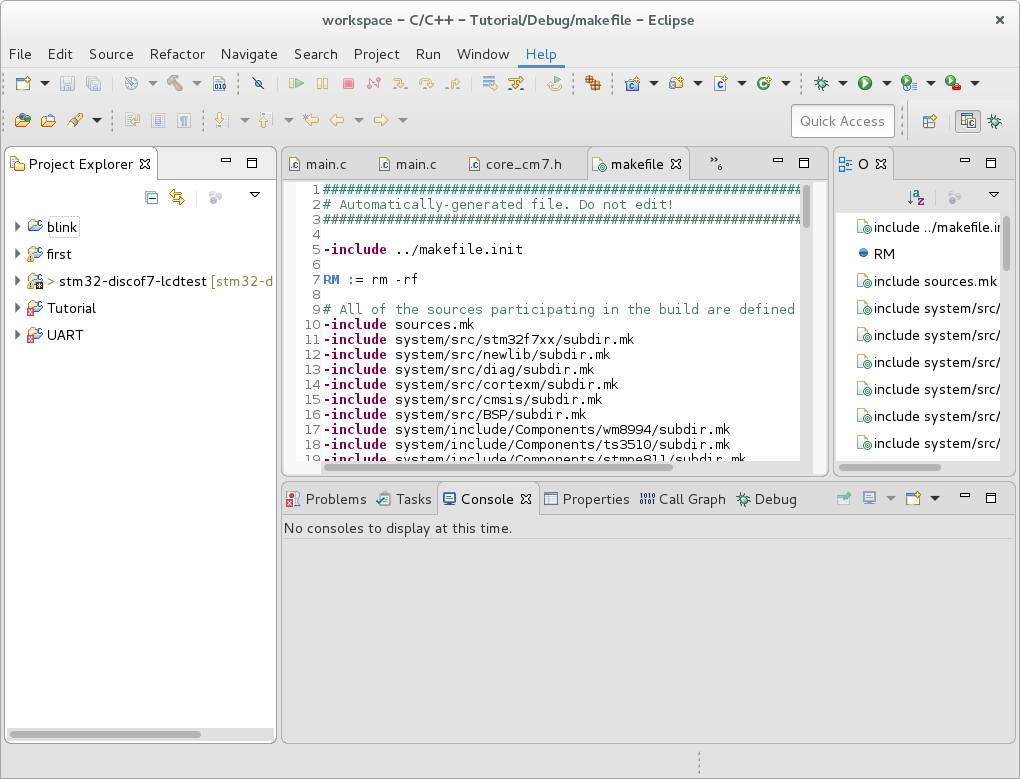
\includegraphics[width=12cm]{grafiken/debugger/EclipseNewSoftware.png}
\label{eclipse_softwareinstallation}
\caption{Eclipse Softwareinstallation}
\end{center}
\end{figure}
Im Fenster 'Install New Software' das Textfeld 'Work with' mit 'GNU ARM Eclipse Plug-ins' füllen. Der richtige Eintrag wird dann vorgeschlagen.
\begin{figure}[h]
\begin{center}
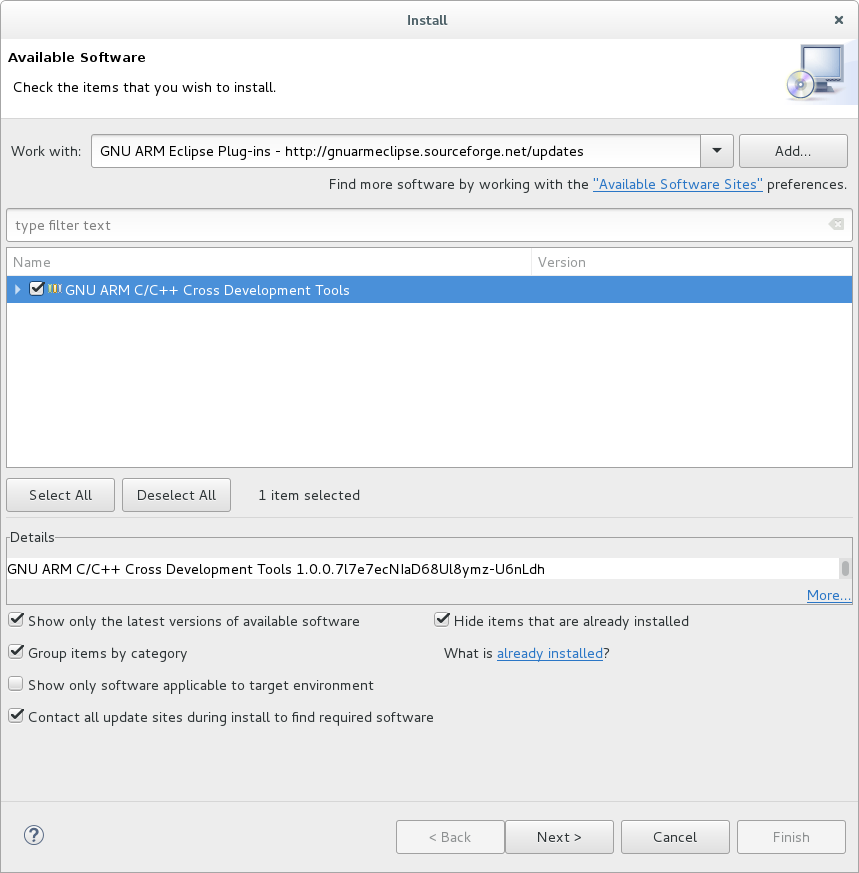
\includegraphics[width=12cm]{grafiken/debugger/GNUauswahl.png}
\label{eclipse_gnu_auswahl}
\caption{Installationsfenster}
\end{center}
\end{figure}
Danach muss der Haken beim Plugin gesetzt werden, ('GNU ARM C/C++ Cross Development Tools') und der Button 'next' betätigt werden. Eventuell muss man jetzt noch ein paar Lizenzverträgen zustimmen. Einfach die Dialoge mit next durchgehen und zum Schluss 'finish' betätigen.
\section{Installieren von OpenOCD}
OpenOCD agiert als GDB-Server in unserer Anwendung. Darum müssen wir diese Anwendung noch installieren.
Zuerst muss wieder das GIT-Repository geklont werden. Wir wechseln dazu zum opt-Ordner in unserer Linux-Distribution.
\begin{lstlisting}
cd /opt
# falls noch nicht vorhanden, muss der Ordner gnuarmeclipse erzeugt werden
sudo mkdir gnuarmeclipse
cd gnuarmeclipse
sudo mkdir openocd
cd openocd
sudo git clone http://openocd.zylin.com/p/openocd.git openocd-stm32f7
cd openocd-stm32f7
# zum bauen folgende Befehle verwenden
sudo ./bootstrap
sudo ./configure --enable-stlink
sudo make -j4
# testen, ob alles funktioniert:
cd tcl
../src/openocd -f board/stm32f7discovery.cfg
\end{lstlisting}
Wir arbeiten im /opt-verzeichnis, da das GNU-ARM-Plug-in Konventionen folgt. Wenn man im Ordner gnuarmeclipse Installationen anlegt, werden diese automatisch vom Plug-in erkannt.
Nichtsdestotroz müssen jetzt in Eclipse Einstellungen angepasst werden.
Bei unserer Lösung des Debuggens wird OpenOCD als externes Tool gestartet. Dazu müssen in Eclipse ein paar Änderungen vorgenommen werden. Unter dem Menüpunkt 'Run'>'External Tools Configurations...' können die Einstellungen hierfür vorgenommen werden.
\begin{figure}[h]
\begin{center}
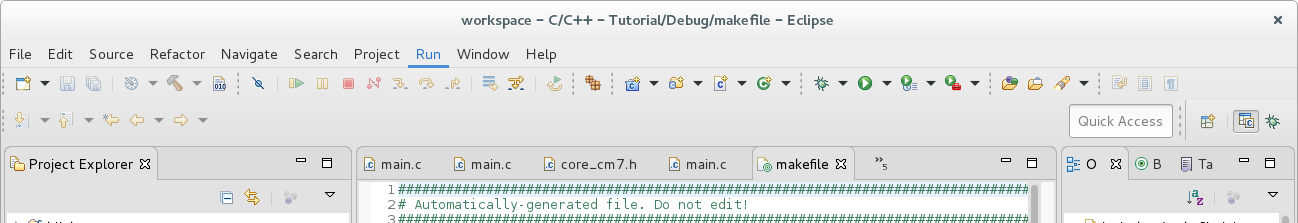
\includegraphics[width=12cm]{grafiken/debugger/RunConfiguration1.png}
\label{eclipse_external_tool_setup}
\caption{Externes Tool einstellen}
\end{center}
\end{figure}
Es müssen dann die Einstellungen wie in \ref{ecplipse_OpenOCD_setting1} vorgenommen werden: 
\begin{figure}[h]
\begin{center}
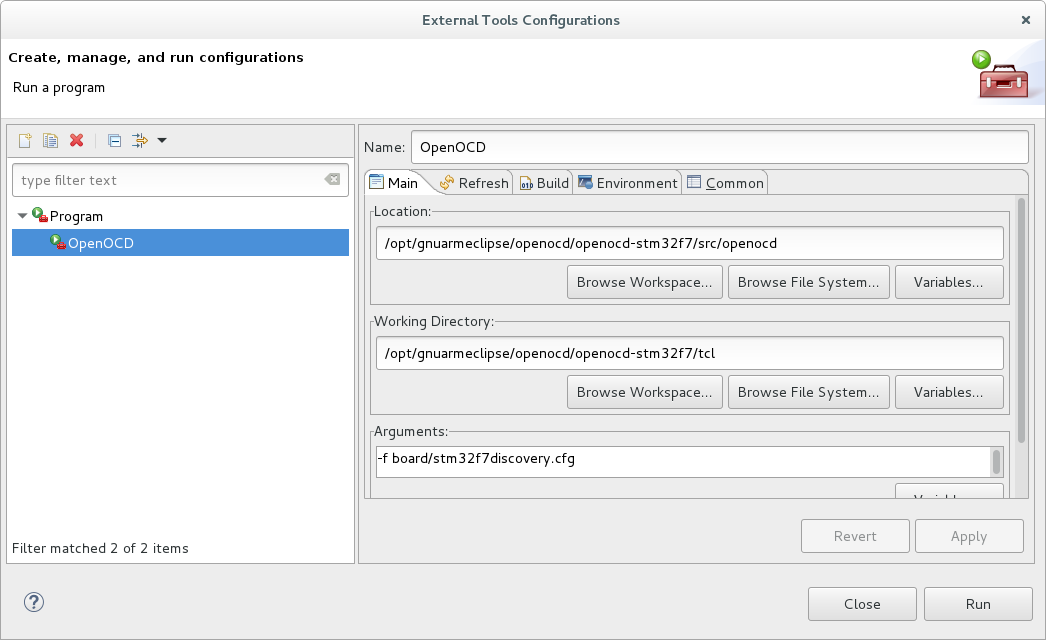
\includegraphics[width=12cm]{grafiken/debugger/OpenOCDsetting.png}
\label{ecplipse_OpenOCD_setting1}
\caption{OpenOCD Settings}
\end{center}
\end{figure}
\newpage
\section{GDB-Setup}
In diesem Kapitel wird das Setup des GDB-Debuggings behandelt. Zuvor haben wir die Toolchain für die Entwicklung auf der Zielplattform heruntergeladen. Nun müssen wir nur noch Eclipse beibringen, wie es den GDB aus der Toolchain findet. Außerdem müssen die passenden Parameter zur Ausführung des GDBs gesetzt werden.
Um in die Debug-Einstellungen zu gelangen, muss im Menüpunkt 'Run' 'Debug Configurations... ' gewählt werden. 
\begin{figure}[h]
\begin{center}
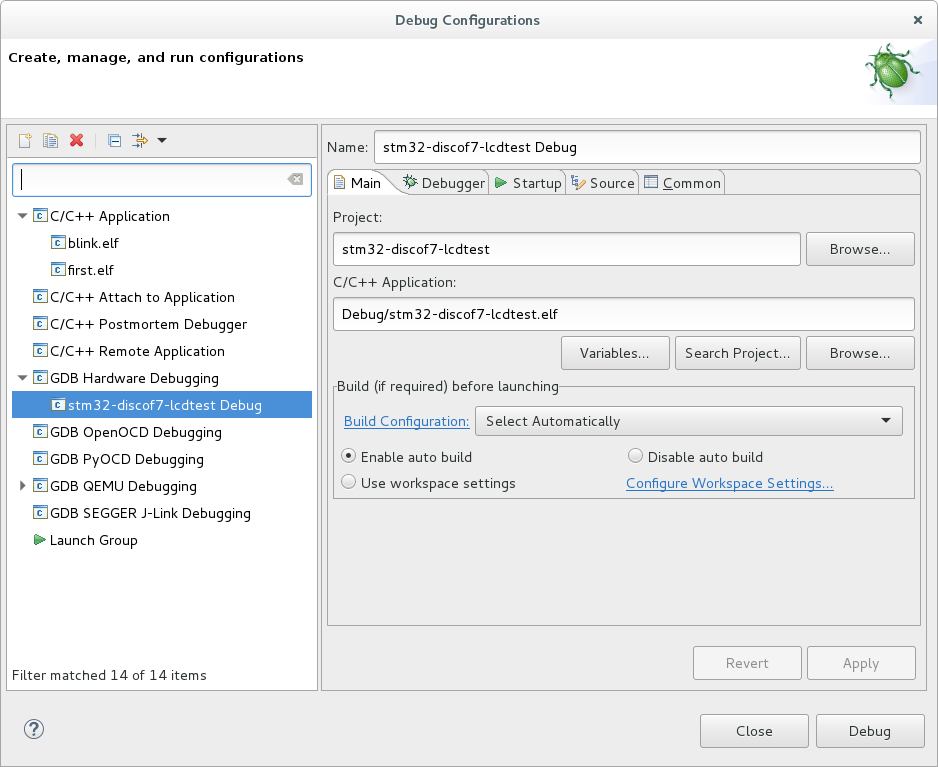
\includegraphics[width=12cm]{grafiken/debugger/GDBsetting1.png}
\label{ecplipse_GDB_setting1}
\caption{GDB Settings}
\end{center}
\end{figure}
Es muss eine neue Konfiguration erzeugt werden, danach werden die Parameter eingetragen. Im Feld Projekt muss der Projektname eingetragen werden, im Feld 'C/C++-Application' der Name des Kompilats.
\begin{figure}[h]
\begin{center}
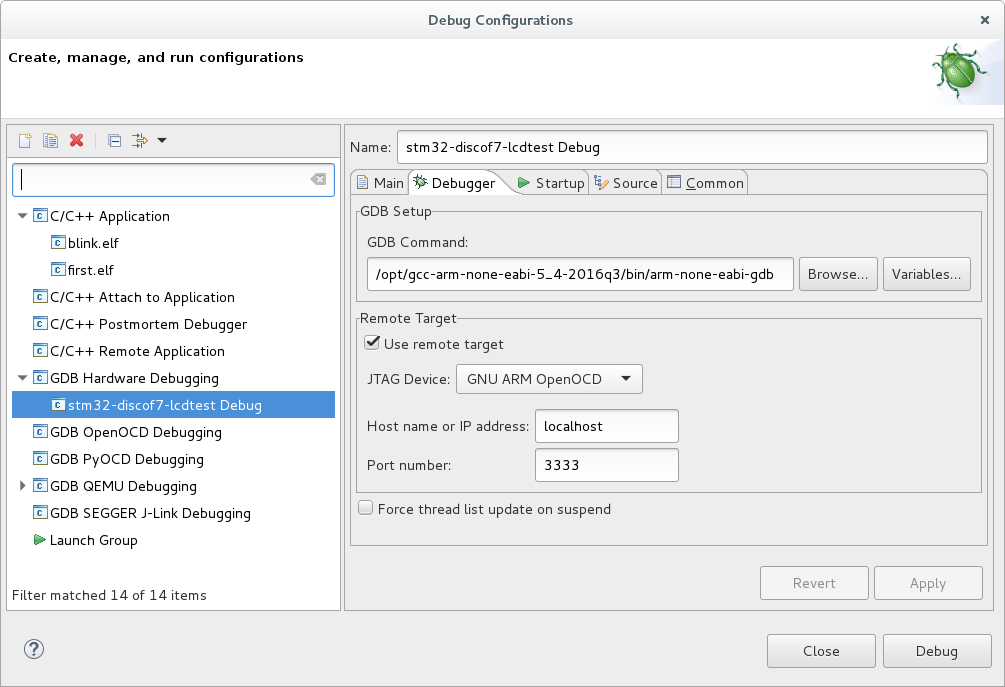
\includegraphics[width=12cm]{grafiken/debugger/GDBsetting2.png}
\label{ecplipse_GDB_setting2}
\caption{GDB Settings 'Debugger'}
\end{center}
\end{figure}
Im Abschnitt 'Debugger' sollte die Konfiguration so aussehen wie in \ref{ecplipse_GDB_setting2}.
\begin{figure}[h]
\begin{center}
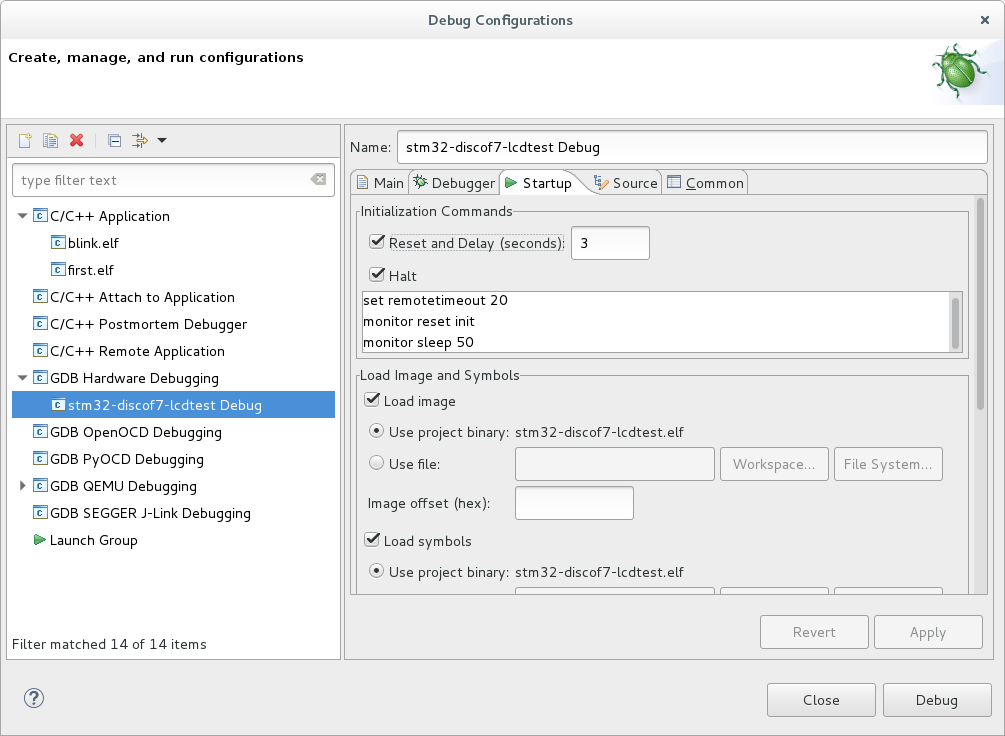
\includegraphics[width=12cm]{grafiken/debugger/GDBsetting3.png}
\label{ecplipse_GDB_setting3}
\caption{GDB Settings 'Startup'}
\end{center}
\end{figure}
Die Startup-Einstellungen müssen noch um die 'Initialization Commands' aus dem Bild \ref{ecplipse_GDB_setting3} ergänzt werden.
'Resume', 'Set breakpoint at: main', 'Load symbols', 'Load image' sind mit einem Haken versehen. 
\FloatBarrier
\section{Debuggen des ersten Projekts}
Um zu debuggen muss zuerst OpenOCD gestartet werden. Dazu muss einfach der Menüpunkt 'Run'>'External Tools'>'<Name der angelegten Konfiguration>' ausgewählt werden. Auf dem Target kann man anhand der blinkenden Status-LED feststellen, dass der Remote-Modus aktiviert wurde. Daraufhin muss der Debug-Button in Eclipse nur noch betätigt werden.
\section{Einsatz des Debuggers}
Als der Debugger bei der Projektarbeit ernsthaft benötigt wurde, setzte das Werkzeug plötzlich aus. Zuerst war es nicht mehr möglich das Projekt auf die Plattform zu befördern und schließlich war es nicht mehr möglich den Debugmodus auf der Hardware zu starten. 
Daraufhin wurde in einem Meeting des Teams besprochen es noch einmal mit einer anderen Installationsanleitung für den Debugger zu versuchen. Zuerst lieferte diese vielversprechende Ergebnisse, jedoch konnte auch hiermit keine Lösung herbeigeführt werden. 
Link zur alternativen Lösung: \url{http://www.carminenoviello.com/2015/01/07/setting-gcceclipse-toolchain-stm32nucleo-part-2/}

\newpage
\documentclass[12pt,a4paper]{article}
\usepackage[utf8]{inputenc}
\usepackage[german]{babel}
\usepackage[T1]{fontenc}
\usepackage{amsmath}
\usepackage{amsfonts}
\usepackage{amssymb}
\usepackage{graphicx}
\usepackage{listings}
\usepackage{color}
\usepackage{hyperref}


\definecolor{dkgreen}{rgb}{0,0.6,0}
\definecolor{gray}{rgb}{0.5,0.5,0.5}
\definecolor{mauve}{rgb}{0.58,0,0.82}

\lstset{frame=tb,
  language=Java,
  aboveskip=3mm,
  belowskip=3mm,
  showstringspaces=false,
  columns=flexible,
  basicstyle={\small\ttfamily},
  numbers=none,
  numberstyle=\tiny\color{gray},
  keywordstyle=\color{blue},
  commentstyle=\color{dkgreen},
  stringstyle=\color{black},
  breaklines=true,
  breakatwhitespace=true,
  tabsize=3
}
\author{Alexander Hebel}
\begin{document}
\section{Portierung von OpnePearl auf den Stm32f7}
Um OpenPearl auf dem Stm32f7 benutzen zu können musste es davor angepasst werden.\\
Für den Microcontroller Lpc1768 wurde bereits ein Portierung gemacht.\\
Diese konnte als Beispielportierung genutzt werden, auch wenn es natürlich Unterschiede zwischen den Microcontrollern gibt, die beachtet werden mussten.\\
Der Lpc1768 beitzt zum Beispiel einen ARM Cortex-M3 und der Stm32f7 einen ARM Cortex-M7.\\
Zudem verfügt der Stm32f7 über ein Farbdisplay welches in unserer Anwendung gut hätte eingesetzt werden können.\\
\\
Um herauszufinden, ob OpenPearl auf dem Stm32f7 läuft sollte ein Testprogramm in pearl geschrieben werden welches eine LED des Microcontrollers blinken lässt.\\
Doch davor musste OpenPearl für den Stm32f7 portiert werden.\\
Im OpnePearl Projekt gibt es einen Ordner runtime.\\
In ihm sind unter anderem die Portierungsdateien für Linux und Lpc1768.\\
Für unsere Portierung wurde der Ordner lpc1768 kopiert, in stm32f7 umbenannt und an unser Zielsystem angepasst.\\
\\
Damit der Ordner stm32f7 bei einem "make install" bearbeitet wird, muss zunächst die Makefile im Ordner runtime angepasst werden, sodass stm32f7 als Target hinzugefügt wird.\\
Die folgende Abbildung zeigt ein Beispiel dieser Änderung.\\
Die komplette Änderung befindet sich im Anhang.\\
\begin{figure}[h]
\begin{center}
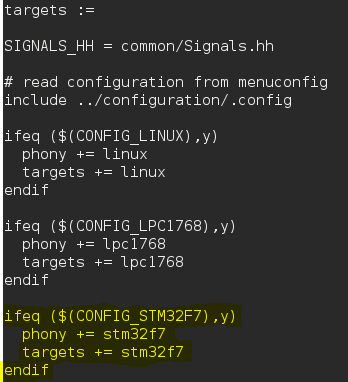
\includegraphics[width=8cm]{grafiken/Makefile_runtime1.png}
\caption{Makefile im Ordner runtime}
\label{Makefile_runtime}
\end{center}
\end{figure}
\newpage
\noindent
Die im Text gelb markierten Stellen wurden neu in die Makefile eingefügt.\\
Mit diesen Änderungen wurde von nun an der Ordner stm32f7 im Ordner runtime bei einem make im Oberverzeichnis berücksichtigt.\\
\\
Nun musste im Ordner smt32f7 alles was mit dem Lpc1768 zutun hatte rausgeschmissen oder ersetzt werden.\\
Zum Beispiel musste die Makefile, die für den Lpc1768 gemacht wurde, auf den stm32f7 abgestimmt werden.\\
Dabei wurde wieder das gleiche Vorgehen wie in der Makefile einen Ordner höher angewandt.\\
Entweder Alles was mit Lpc1768 zu tun hat auskommentierten, oder stm32f7 spezifisch ersetzen.\\
In der Makefile wurde ein Includepfad(../cortexM/stm32f7HAL/Inc) für dem stm32f7 eingefügt.\\
Als Include wurde die HAL-library eingesetzt, in der unter anderem ein Treiber für den I2C des stm32f7 enthalten ist.\\ 
Die folgende Abbildung zeigt einen Teil Änderungen der Makefile im Ordner stm32f7.\\
Die Komplette Änderung befindet sich im Anhang.\newpage
\begin{figure}[h]
\begin{center}
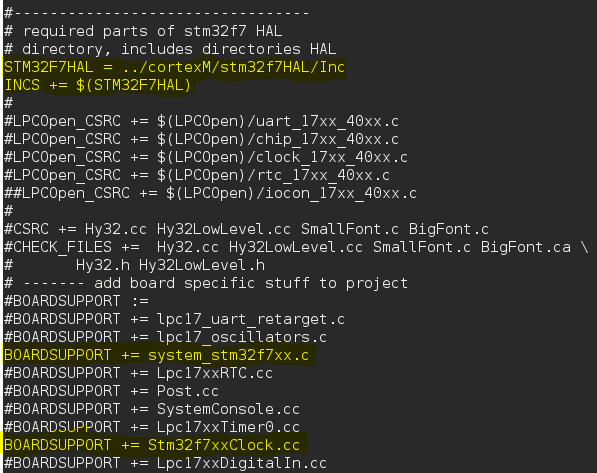
\includegraphics[width=13cm]{grafiken/Makefile_stm32f7_1.png}
\caption{Makefile im Ordner stm32f7}
\label{Makefile_stm32f7}
\end{center}
\end{figure}
\noindent
Des Weiteren wurden die Dateien {\textit{system\_stm32f7xx.c}}, {\textit{Stm32f7xxClock.cc}} und {\textit{startup\_stm32f4xx.S}} als Boardsupport angegeben.\\
Diese Dateien mussten natürlich vorhanden oder neu erstellt werden.\\
Die {\textit{startup\_stm32f4xx.S}} ist eine Vorbereitung für den Microcontroller, die vor dem Laufen eines Programms durchgeführt wird.\\ 
Die {\textit{system\_stm32f7xx.c}} ist für Registerdeclerationen, Bitdeclerationen und Macros um auf Register der Hardware zugreifen zu können.\\
\\
\newpage
\noindent
Im Ordner tests befinden sich Test- und Beispielprogramme.\\
Die Datei Makefile.inc beschreibt, welche Testprogramme bei einem Makebefehl durchgeführt werden.\\
In der Makefile.inc wurden alle Tests des Lpc1768 herausgenommen und ein neuer Test für unser Blinkprogramm(digitaliotest.cc) eingetragen.\\
\begin{figure}[h]
\begin{center}
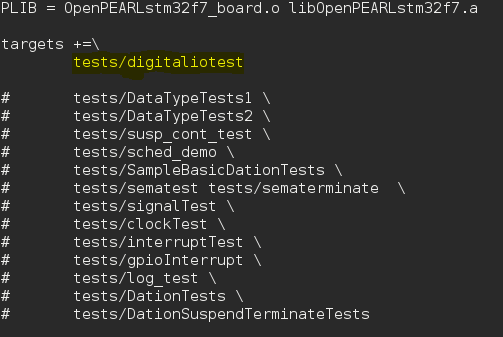
\includegraphics[width=12cm]{grafiken/Makefile_tests.png}
\caption{Makefile im Ordner tests}
\label{Makefile_tests}
\end{center}
\end{figure}
\\
Die mit Raute markierten Zeilen sind Kommentare.\\
Der Name digitaliotest.cc kommt daher, dass es diesen Test schon beim Lpc1768 gab und Teile des Programms für die Blinkyanwendung übernommen wurden.\\
\\
Bei einem make-install-Befehl im obersten Verzeichnis wird nun unter anderem die Datei Pearlincludes.h erstellt und das Programm digitaliotest durchgeführt.\\
Um nicht jedes Mal aufs neue einen Makebefehl durchführen zu müssen änderten wir das prl-Skript.\\ 
Der stm32f7 wurde als neues target eingefügt.\\
Nun konnte man ganz leicht mit dem Befehl {\textit{prl -b stm32f7 digitaliotest.cc}} aus der C++-Datei eine ausführbare Datei generiert werden.\\
Mit dem Befehl {\textit{objcopy -O binary -I elf32-little digitaliotest test.bin}} wurde die Datei digitaliotest.elf in die Datei test.bin(Binärdatei) umgewandelt.\\
Zuletzt wurde die Datei test.bin mit dem Befehl {\textit{st-flash write test.bin 0x8000000}} auf das Board geladen.\\
\\
Doch anders als im Programm vorgesehen, blinkte die angesteuerte LED nicht.\\
Hierfür kann es viele Gründe geben.\\
Es kann sein das FreeRTOS nicht richtig läuft oder ein anderer Aspekt bei der Portierung übersehen wurde.\\
Da der Debugger nicht richtig funktionierte war es schwierig genaueres in Erfahrung zu bringen.\\
\end{document}

\newpage
\section{Das Scheitern der Portierung auf den STM32F746 DISCO}
Einer der Gründe war wie schon bemerkt das Scheitern bei dem Umgang mit dem Debugger. Durch den fehlenden Debugger war es nicht möglich, den geschriebenen Code zu analysieren. Im Klartext bedeutet das, dass nicht festgestellt werden konnte, ob FreeRTOS richtig lauffähig war/richtig konfiguriert war. Da FreeRTOS das Grundgerüst für OpenPEARL darstellt, ist die Sicherstellung der Funktionstüchtigkeit aber zwingend notwendig. Um die Überprüfung des Shedulers durchführen zu können, muss man in der Lage sein, den Prozessor zu stoppen, Zwischenergebnisse, Registerinhalte anzeigen zu können, zu sehen, in welcher Zeile des Quellcodes man sich gerade befindet. Und ebendies war wegen dem Fehlen des Debuggers nicht möglich. 
Des Weiteren wurde festgestellt, dass die Toolchain, die im Projekt Verwendung fand vom Funktionsumfang her nicht geeignet war. 
Der Kompiler konnte Dinge nicht, die zum Übersetzen erforderlich waren. Eine Funktion, die der verwendeten Kompilerversion beispielsweise fehlt, ist die Funktion Link Time Optimization. Diese wird benötigt, um die Größe des Kompilats zu minimieren oder klein zu halten. Jedoch dürfte dies nicht wirklich das Hauptproblem des Scheiterns gewesen sein, da unser Target, der STM32 über genügend Speicher verfügt. 
Zu allem Übel kam hinzu, dass dem Team die Zeit knapp wurde. Bis Anfang Dezember konnten keine großartigen Ergebnisse geliefert werden, was auch dazu führte, dass die Lust am Projekt und an der Beteiligung drohte abzunehmen. 
Aus diesem Grund wurde an einer Sitzung im Dezember besprochen, wie weiter fortzufahren ist. Das Team wurde sich einig über ein Alternativprogramm.
Die Alternative sieht eine zweigleisige Entwicklung vor. Ein Teil des Teams befasst sich mit der Entwicklung der ursprünglich angedachten Anwendung. Diese Anwendung ist wichtig, da sie bei der Präsentation gegen Ende des Semesters das Projekt von einem rein theoretischen Ansatz her mit der Praxis verbindet. Die Anwendung soll auch darstellen, dass OpenPEARL wirklich funktioniert und praxistauglich ist. Die zweite Schiene der Entwicklung befasst sich mit der Entwicklung eines I2C-Treibers für das Microcontrollerboard LPC1768, das teilweise vom OpenPEARL-Projekt bereits Unterstützung fand. Beispielsweise waren schon Treiber für die Benutzung des Displays mit unterschiedlichen Schriftarten vorhanden.

\newpage

\section{Programmieren der Anwendung}
Aus Zeitgründen musste die Portierung des Stm32f7 abgebrochen werden.\\
Deshalb wurde die Anwendung für den RaspberryPi geschrieben.\\
Um mit der Kugelmaschine kommunizieren zu können stand ein $I^2$C-Teil für den RaspberryPi bereit.\\
Doch bervor man direkt an das Programmieren der Anwendung gehen konnte, war ein wenig Einarbeitung in die Programmiersprache OpenPearl nötig.\\
\subsection{Vorbereitung}
Um in die Syntax von OpenPearl hinein zu finden und das Semaphorenwissen wieder ein bisschen aufzufrischen war es zunächst die Aufgabe das Erzeuger-Verbraucher-Problem(Liteartur:  Rainer Oechsle, {\textit{Parallele Programmierung mit Java Threads}}, 2001) in OpenPearl zu programmieren.\\
Als das erledigt war, folgte das Philosophen-Problem(Liteartur: K. Mani Chandy \& Jayadev Misra, {\textit{The Drinking Philosophers Problem}}, 1984).\\
Hierbei fiel vor allem auf, wie leicht das Programmieren mit OpenPearl von der Hand geht.\\
Für diese beiden Aufgaben wurde im Vergleich zu anderen Programmiersprachen, wie zum Beispiel Java, nur sehr wenig Zeilencode benötigt.\\
Dadurch, dass man das Programm in Tasks strukturiert, wird es automatisch übersichtlicher.\\
Beispielsweise macht man sich einen Task für die Ausgabe und einen für den Algorithmus.\\
Nachdem das Philosophen-Problem erledigt war, konnte mit der richtigen Anwendung gestartet werden.\\
Dabei wurde der Rechner mit dem RaspberryPi und der RaspberryPi über $I^2$C mit der Kugelmaschine verbunden.\\
\newpage
\begin{figure}[h]
\begin{center}
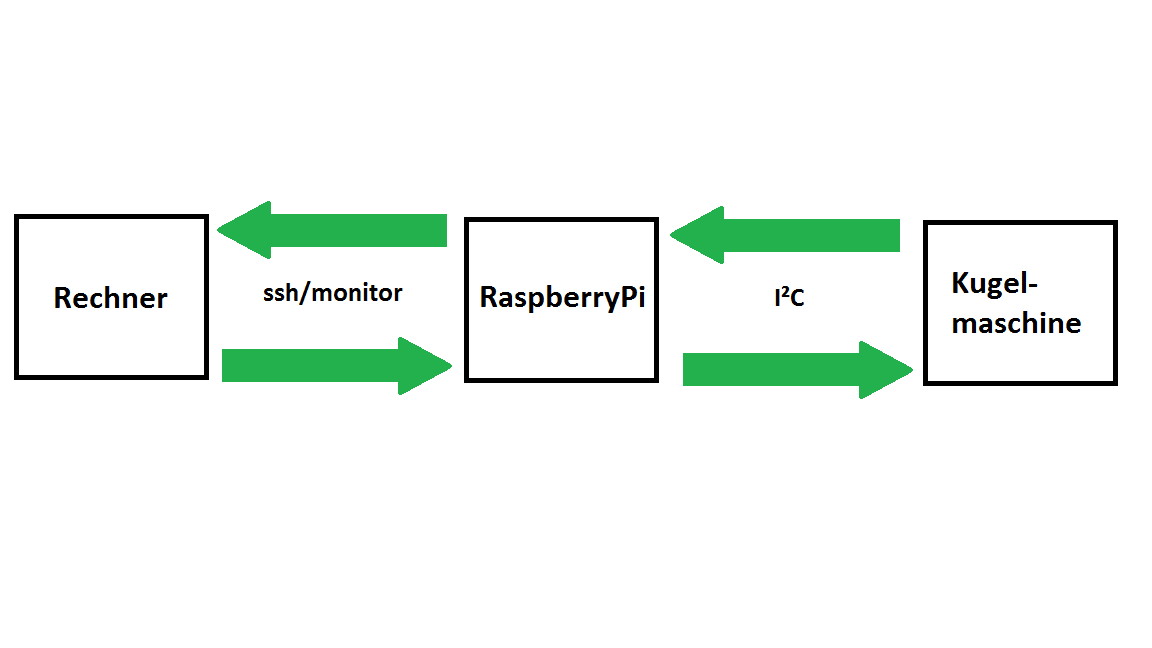
\includegraphics[width=15cm]{grafiken/Kommunitations_schema.png}
\caption{Kommunikationsschema}
\label{Kommunikationsschema}
\end{center}
\end{figure}
\noindent
Zunächst wurde versucht jedes einzelne Gerät (Motor, Lichtschranke, Klappen, Waage) der Kugelsortiermaschine anzusteuern.\\
Man konnte schnell erkennen, dass viele Semaphoren für die Sortierung nötig waren, da die Kugel immer nur weiter rollen darf, wenn der nächste Abschnitt, in den sie rollt, frei ist.
In Teilen des Programms musste C bzw. cpp Code verwendet werden, da manche Funktionen (z.B. Auslesen eines einzelnen Bits) noch nicht in OpenPearl umgesetzt sind.\\
Beim Testen des Motors fiel auf, dass die analogen Werte sich ab einem bestimmten Durchmesser nicht mehr änderten.\\ 
Durch die Anpassung eines Wertes bei der Initialisierung des Analog-Digital-Converter(ADC) konnte dieser Fehler jedoch behoben werden.\\
\newpage

\subsection{Gerätesteuerung}
\subsubsection{Lichtschranken}
Die Kugelsortiermaschine besitzt insgesamt 9 Lichtschranken.\\
In unserer Anwendung sind die Lichtschranken so durchnummeriert, dass Lichtschranke 1 die oberste im Bau der Maschine ist und Lichtschranke 9 ganz unten links zu finden ist.\\
Die Nummern der Lichtschranken sind also von oben nach unten durchnummeriert.\\
Über den eingesetzten $I^2$C-Portexpander können aber nur maximal 8 Bit übertragen werden.
Deshalb erstellt man eine neue Variable “ls“ und hängt dem 8 Bit Block ein einzelnes Bit an.\\
\begin{lstlisting}
TAKE b8 FROM uls1_8;
TAKE b1 FROM uls9;
__cpp__('ls = _b1.bitCat(_b8);');
\end{lstlisting}
Somit enthält die Variable “ls“ den Status aller neun Lichtschranken.\\
Um aus dieser Variable den Wert einer Lichtschranke heraus zu lesen benötigt man wieder C-Code.\\
\begin{lstlisting}
DCL l1 BIT(1);
__cpp__('_l1 = _ls.getBit(9);');
\end{lstlisting}
In der Kugelsortieranwendung fragt der TASK readInputs alle 1/10 Sekunden die Werte der Lichtschranken neu ab.\\
\clearpage
\subsubsection{Dickenmessplatz}
Der Motor wird in der Kugelsortieranwendung dazu benutzt den Durchmesser einer Kugel zu bestimmen. Man kann ihm die drei Signale auf, zu oder stopp senden.\\
Des Weiteren kann man über zwei boolean Variablen auslesen, ob der Motor zu oder offen ist.\\
Da der Motor beim Zufahren nicht automatisch anhält wenn er geschlossen ist, sondern verklemmt, sorgte am Anfang für Verwirrung.\\
In der Sortieranwendung wird die Rolle des Motors im Task motor gemanaged.\\
Es gibt eine Variable Status die sich entweder im Zustand öffnend, schließend oder geschlossen befindet.\\
Um Verklemmung des Motors zu vermeiden wird die Polling-Methode mit kurzen Wartepausen(100ms) angewendet.\\
Das bedeutet es wird so lang in kurzen Zeitintervallen abgefragt ob der Motor offen bzw. geschlossen ist, bis das Ereignis zutrifft.\\
\newpage

\subsubsection{Klappen}
Insgesamt besitzt die Kugelsortiermaschine 7 Klappen bzw. Stoßer.\\
Um eine einzelne Klappe anzusprechen hätte wieder C-Code eingefügt werden müssen, doch dies war für unsere Anwendung nicht nötig.\\
Somit wurden immer auf alle Klappen geschrieben um sie auf oder zu zumachen.\\ 
Wie die Lichtschranken auch wurden die Klappen für unser Programm von oben nach unten durchnummeriert, sodass Klappe1 ganz oben und Klappe7 ganz unten links liegt.\\
Um zum Beispiel Klappe1 zu öffnen wurde das Bit 0000001 auf uhm1-7 gesendet.\\
\begin{lstlisting}
DCL (k1,allOff) BIT(7) INIT('0000001'B1, '0000000'B1);
SEND k1 TO uhm1_7;
AFTER 1 SEC RESUME;
SEND allOff TO uhm1_7;
\end{lstlisting}
Will man zwei Klappen gleichzeitig öffnen benötigte man jediglich ein anderes Bitmuser.\\
Zum Beispiel Klappe1 und Klappe2 :
\begin{lstlisting}
DCL test BIT(7) INIT('0000011' B1);
\end{lstlisting}
\subsubsection{Waage}
Genauso wie der Motor liefert die Waage in unserer Anwendung den analogen Wert für das Gewicht der Kugeln in Gramm.\\
Nachdem die Dichte ausgerechnet wurde, wird die Kugel von der Waage weggestoßen und je nach Dichte eine unterschiedliche Klappe geöffnet.\\
Das \nameref{Sortierkriterium} und die \nameref{Umrechnung analoger Werte} befinden sich in späteren Kapiteln.\\
\clearpage

\subsection{Sortierkriterium}\label{Sortierkriterium}
Anfangs war das Sortierkriterium ausschließlich der Wert der Dichte.\\
Doch bei Tests stellte sich heraus, dass die Klappe ganz rechts(Draufsicht) sich nicht vollständig öffnen ließ.\\ 
Wahrscheinlich weil die Maschine lange nicht in Benutzung war.\\
Es stellte sich jedoch heraus, dass kleine Kugeln dennoch durch die Öffnung passten.\\
Deshalb änderten wir das Sortierkriterium um jede Klappe auszunutzen.\\
Eine Kugel fällt in die 1. Schiene (Draufsicht ganz rechts), wenn ihr Durchmesser kleiner als 1.5cm ist.\\
Ist die Dichte einer Kugel kleiner 1 g/$cm^3$ wird sie in die 2. Schiene (Draufsicht eins weiter links) sortiert.\\
Eine Kugel fällt in die 3. Schiene, wenn ihre Dichte kleiner 2 g/$cm^3$ und größer 1 g/$cm^3$ ist.\\
In die 4. Schiene fällt eine Kugel mit einer Dichte kleiner 4 g/$cm^3$ und größer 2 g/$cm^3$.\\
Hat eine Kugel eine Dichte größer 4 g/$cm^3$ fällt sie in die 5. Schiene.\\ 
\newpage

\subsection{Umrechnung analoger Werte}\label{Umrechnung analoger Werte}
In der TASK rechner wird die Dichte der Kugel berechnet.\\
Um die Dichte auszurechnen benötigt man das Volumen und für das Volumen benötigt man den Durchmesser und das Gewicht der Kugel.\\
Die Machine liefert nur einen analogen Wert.\\
Das bedeutet man muss aus dem analogen Wert den realen Wert errechnen.\\
\\
In eine Excel Tabelle wurden die Analogen und realen Werte Aufgeschrieben, und der Faktor errechnet.\\
Zum Schluss wurde für das Gewicht und dem Durchmesser ein Durchschnittsfaktor errechnet.\\
\begin{figure}[h]
\begin{center}
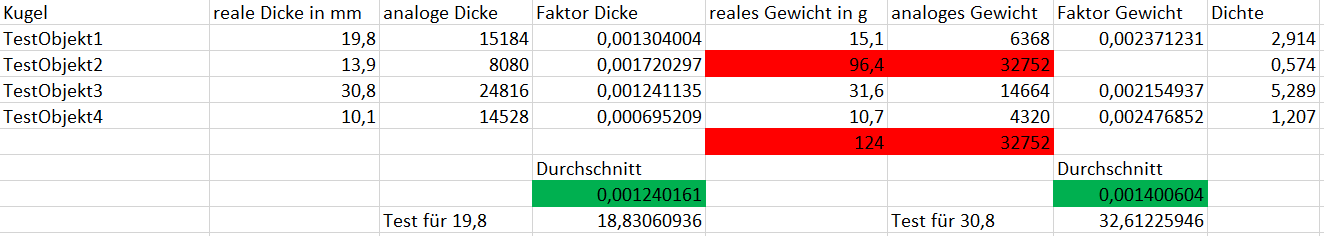
\includegraphics[width=15cm]{grafiken/UmrechnungsTabelle.png}
\caption{Umrechnung - Tabelle}
\label{Umrechnung}
\end{center}
\end{figure}
\\
Ein Wert für das Gewicht konnten wir nicht nutzen, da das analoge Gewicht ab einem bestimmten Gewicht gleich groß blieb.\\
Am Ende wurde mit den neuen Faktoren die Dichte von ein paar Kugeln berechnet.\\
\begin{figure}[h]
\begin{center}
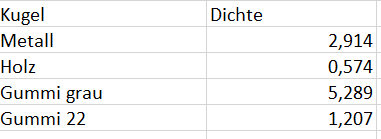
\includegraphics[width=10cm]{grafiken/UmrechnungTests.png}
\caption{Umrechnung - Tests}
\label{Umrechnung}
\end{center}
\end{figure}
\newpage




\subsection{Programmfluss}
Der Programmfluss wird durch 14 Semaphoren geregelt.\\
Um dies zu veranschaulichen ist im Anhang ein \nameref{Aktivitätsdiagramm} beigelegt.\\
In diesem ist jede Semaphore unterschiedlich eingefärbt, damit gleiche Semaphoren in unterschiedlichen Tasks besser erkennbar sind.\\
\\
Das Programm besteht aus 6 Tasks.\\
Die Main Task dumpInputs aktiviert die anderen 5 Tasks und kümmert sich anschließend nur noch um die Ausgabe.\\
\\
Der Task motor regelt den Zugriff zum Durchmesser lesen.\\
Bevor der Durchmesser gelesen werden darf, fordert der Task die Semaphoren motorgo und durchmesserlesen an.\\
Die semaphore motorgo prüft ob sich der Wert der Lichtschranke vor dem Motor geändert hat.\\
Falls ja wird sie auf true gesetzt.\\
Die Semaphore durchmesserlesen prüft ob die letzte Kugel von der Waage gestoßen wurde.\\
Sie wird beim Starten des Programms mit true initialisiert und sonst beim stoßen von der Waage befreit.\\
Nachdem der analoge Durchmesserwert gelesen wurde, wird die Semaphore mesdu befreit.\\
Sie bewirkt, dass im Task rechner aus dem analogen Wert der reale Durchmesser berechnet werden darf.\\
Anschließend wird die Semaphore waagefrei angefordert um sicher zu gehen, dass sich auf der Waage keine Kugel mehr befindet.\\
Zuletzt wird die Semaphore beginn freigeben, was dazu führt, dass wieder eine neue Kugel vom Start gestoßen werden kann.\\
Zudem wird die Semaphore Motorklappe freigegeben, damit nicht gleichzeitig auf unterschiedliche Klappen zugegriffen werden kann.\\
\\
Die Klasse readinputs kümmert sich um das einlesen der Lichtschranken.\\
Sie befreit die Semaphore motorgo, wenn sich der Wert der Lichtschranke vor dem Motor ändert.\\
Des weiteren bestätigt der Task das Sortieren, da sie die Lichtschranken in der Sortierrinne abfrägt.\\
\\
Der Task stoßer ist für die Steuerung der Waage verantwortlich.\\
Sobald der analoge Gewichtswert genommen wurde, wird die Semaphore mesgew befreit, sodass im Task rechner das reale Gewicht berechnet werden kann.\\
Danach wird die Semaphore stossen verlangt, welche nach dem errechne der Dichte der Kugel freigegeben wird.\\
Nachdem die Kugel weggestoßen wurde, wird die Semaphore durchmesserlesen befreit, sodass der Durchmesser der nächsten Kugel gelesen werden kann.\\
Sobald die Kugel in der richtigen Sortierrinne gelandet ist und an der Lichtschranke der Sortierrinne vorbeigerollt ist, schließen sich wieder alle Klappen.\\
Zuletzt wird die Semaphore waagefrei released, damit die nächste Kugel in die Waage rollen kann.\\
\\
Der Task rechner kümmert sich jeweils nur darum den realen Durchmesser,Gewicht und Dichte zu berechnen.\\
Er wartet durch Semaphoren darauf, dass neue analoge Werte geliefert werden und rechnet diese dann um.\\
\\
Der gesamte \nameref{Quellecode} des Programms befindet sich in unserem Repository.\\ 
\newpage




\subsection{Ausgabe}
Um den Kontrollfluss besser nachvollziehen zu können wurde eine Ausgabe entwickelt.
Die Komplette Ausgabe baut auf den Steuerzeichen der vt100 Konsole auf.\\
In der Main Task wird gleich zu Beginn ein Schema aufgebaut, dass sich danach nur bei Änderung ändert.
Diese zeigt die wichtigsten Daten in einer Tabelle an.\\
Wie zum Beispiel den ungefähren Aufenthalt der Kugel und enthält die Dichte der bisher sortierten Kugeln.\\
Auf der linken Seite der Ausgabe befindet sich die Tabelle.\\
\begin{figure}[h]
\begin{center}
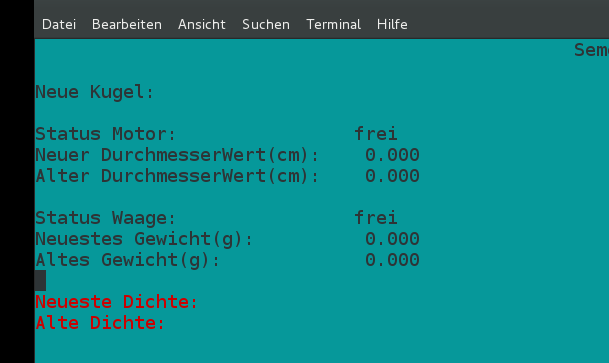
\includegraphics[width=10cm]{grafiken/Ausgabe_tabelle.png}
\caption{Ausgabe - Tabelle}
\label{Ausgabe}
\end{center}
\end{figure}
Sie enthält den Status, ob eine neue Kugel eingefügt werden kann, ob der Motor und Waage frei sind oder nicht, den Wert des letzten Durchmessers, Gewicht, und Dichte, den Wert des neuen Durchmessers, Gewicht und Dichte.
\newpage
\noindent
Auf der rechten Seite der Ausgabe befindet sich ein Schema der Maschine.
\begin{figure}[h]
\begin{center}

\includegraphics[width=10cm]{grafiken/Ausgabe_Schema.png}
\caption{Ausgabe - Schema}
\label{Ausgabe}
\end{center}
\end{figure}
Die X'se stellen den Weg der Kugelsortiermaschine dar.\\
Das Zeichen '<-' stellt den Stoßer ganz am Anfang der Kugelsortierung dar.\\
Durch das Zeichen '-| X |-' soll der Motor dargestellt werden.\\
Und das Zeichen 'T' soll die Waage symbolisieren.\\
Falls die Kugel sich an einem bestimmten Punkt in der Sortierung befindet, wird das X durch einen roten Kreis ersetzt.\\
\begin{figure}[h]
\begin{center}
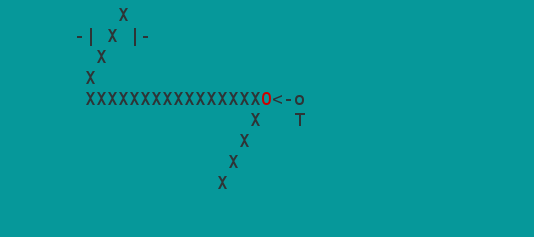
\includegraphics[width=10cm]{grafiken/Ausgabe_KugelinWaage.png}
\caption{Ausgabe - Waage}
\label{Ausgabe}
\end{center}
\end{figure}
\newpage
\noindent
Ganz unten in der Ausgabe befindet sich wieder eine Tabelle mit 5 Spalten.
Diese 5 Spalten symbolisieren die Rinnen in denen Die Kugel sortiert wird.
\begin{figure}[h]
\begin{center}

\includegraphics[width=14cm]{grafiken/Ausgabe_sortierte.png}
\caption{Ausgabe - Sortierung}
\label{Ausgabe}
\end{center}
\end{figure}
Der Kreis soll eine Kugel darstellen und daneben ist die Dichte angegeben mit der die Kugel sortiert wurde.
Die Werte der Kugeln stapeln sich in der Tabelle untereinander auf, so wie sie es auch in der Kugelsortiermaschine machen. 
\newpage

\subsection{Noch Fehlend}
Die Anwendung besitzt keine Fehlerbehandlung und auch die Ausgabe ist noch verbesserungswürdig.\\
Wenn zum Beispiel keine Kugel im Motor ankommt fährt dieser trotzdem zu und das Programm geht weiter.\\
Man müsste in diesem Fall das Programm anhalten und wieder zurücksetzten.\\
Genauso ist es ein Fehler, wenn die Kugel irgendwo hängen bleibt oder einfach nicht weiter rollt.\\
Hierzu könnte man nach jeder Lichtschranke oder zumindest an den kritischen Stellen nach einer bestimmten Zeitüberschreitung, einen Fehler ausgeben.\\
Diese ganze Fehlerbehandlung könnte dann noch in die Ausgabe eingebaut werden, damit Fehler sofort erkannt werden und behoben werden können.\\
Auch der Zugriff auf die Klappen ist noch nicht optimal, da immer auf alle Klappen zugegriffen wird.\\
Sicherer wäre es immer nur einzelne Klappen anzusprechen.\\
In unserer Anwendung wurden Semaphoren benutzt um zu verhindern, dass gleichzeitig auf unterschiedliche Klappen zugegriffen wird.\\
Diese Semaphoren würden dadurch entfallen und den Programmfluss einfacher gestalten.\\  








\newpage
\chapter{Installation der Tools für die Entwicklung mit dem LPC1768}
\sectionauthor{Autor: Jonathan Weißenberger}
Bei der Entwicklung wird weiterhin mit einer virtuellen Maschine gearbeitet. Als Betriebssystem kommt Debian zum Einsatz. Während der Entwicklung des Treibers wurde festgestellt, dass Virtal Box von Oracle als Virtualisierungsumgebung nicht eignet. Es kann bei der Kommunikation mit dem Entwicklungsboard über USB zu Verzögerungen kommen.
Um überhaupt arbeiten zu können wurde das OpenPEARL-Projekt von SourceForge erneut geklont. Zudem wird eine funktionierende Toolchain benötigt. In unserem Projekt kommt nach Absprache mit unserem betreuenden Professor Herr Müller Version {\textit{gcc-arm-none-eabi-4\_9-2014q4}}
 zum Einsatz. 
Die Version {\textit{gcc-arm-none-eabi-5\_4-2016q3}}
 erwies sich beim ersten Projektansatz- dem Versuch OpenPEARL für den STM zu portieren als fehlerhaft und unvollständig. Durch die Erfahrung des Professors Herr Müller konnte schnell die passende Version gefunden werden.
Bei der weiteren Installation wird die Anweisung von \url{https://sourceforge.net/p/openpearl/wiki/Microcontroller%20Runtime%20System%20Environment/} befolgt. Es muss ein Flash-Tool für den LPC heruntergeladen und installiert werden. Zum Einsatz kommt \textit{lpc21isp}. Heruntergeladen wird das Tool von \url{https://www.segger.com/downloads/jlink} als Debian Package. Mittels 
\begin{lstlisting}
sudo dpkg -i <Name des heruntergeladenen Packages>
\end{lstlisting}
wird das Paket dann installiert. //
Daraufhin muss die zugehörige udev-Rule für das Microcontrollerboard eingetragen werden. Dazu wird die Datei \textit{88-openpearl.rules} angelegt.
\begin{lstlisting}
sudo vim /etc/udev/rules.d/88-openpearl.rules
\end{lstlisting}
In der Datei müssen folgende Einträge erfolgen:
\begin{lstlisting}
SUBSYSTEMS=="usb", ATTRS{idVendor}=="0403", ATTRS{idProduct}=="6001", GROUP="users", MODE="0666"
SUBSYSTEMS=="usb", ATTRS{idVendor}=="1366", ATTRS{idProduct}=="0101", GROUP="users", MODE="0666"
\end{lstlisting}
Zuletzt wird ein Logger oder Visualisierungstool für die ankommenden Daten vom UART benötigt. Hierzu wird Minicom installiert.
\begin{lstlisting}
sudo apt-get install minicom
\end{lstlisting}

\chapter{I2C Treiber LPC1768}
\sectionauthor{Autor: Jonathan Weißenberger}
\section{Voraussetzungen für den Treiber}
Um beim gesamten OpenPEARL-Projekt den Wartungsaufwand zu minimieren haben sich die Entwickler bei der Umsetzung auf ein modulares System entschieden. Das bedeutet, wenn ein hardwarespezifischer Treiber gebraucht wird, müssen nur die verfügbaren Interfaces implementiert werden und an einer anderen Stelle der Treiber bekannt gemacht werden und schon ist das Gerät verwendbar. Die bereits bestehenden FreeRTOS oder Linux-Module greifen dann auf die spezifizierten Interfacefunktionen zu. 
Die Interfaces, die für den I2C-Treiber implementiert werden mussten beschränken sich auf eines - das 'I2CProvider'-Interface.
\section{Vorgehensweise}
Bei der Programmierung wurde als Referenz eine Demoapplikation des Herstellers hergenommen. Bei der Applikation wurde jedoch für eine andere Zielplattform entwickelt. Da jedoch die Funktionsbezeichner für unterschiedliche Boards bei den Herstellern ziemlich ähnlich sind, konnte das Beispiel eine gute Hilfestellung bieten. Es wurde klar, welche Funktionsaufrufe üblich und gefordert sind um das richtige Pinverhalten der I2C-Pins zu bekommen. Und überhaupt die Information über vorhandenes Pin-Muxing wurde geliefert. Darüberhinaus stellten sich auch schnell Unterschiede zu den Targets, die LPC11xx, für welche die Referenz verfasst ist, heraus.
\section{Wesentliche Bestandteile des Treibers}
Alle verwendeten Interfacedefinitionen von OpenPEARL befinden sich im Ordner {\textit{/runtime/common}}.
Der beim Projekt eingesetzte I2CProvider besitzt 3 Methoden, die im Treiber umgesetzt werden müssen.
\begin{lstlisting}
virtual int readData(int adr, int n, uint8_t * data) = 0;
virtual int writeData(int adr, int n, uint8_t * data) = 0;
virtual void rdwr(int n, I2CMessage* data) = 0;
\end{lstlisting}
Um in der Interrupserviceroutine abfragen zu können, ob der Lese-/ oder Schreibvorgang vom Gerät schon beendet wurde, musste in der Bibliothek des I2Cs des LPC1768 eine Funktion ergänzt werden. Alle Bibliotheken der unterstützten Boards basierend auf Cortex-Chips können in {\textit{/runtime/cortexM/}} gefunden werden.
\begin{lstlisting}
INLINE int getStatus(I2C_ID_T id){
	return (int)i2c[id].mXfer->status;
}
\end{lstlisting}
Im wesentlichen ermöglicht die Funktion das Auslesen des Status der I2C-Einheit. 

\section{Beschreibung des Konstruktors}
Der Konstruktor enthält logischerweise mehrere Aufrufe auf die Treiber des LPC1768. Zuerst muss abhängig von der übergebenen PIN-Id das Pin-Muxing richtig betrieben werden. Das Target LPC1768 besitzt drei unterschiedliche I2C-Busse, die unabhängig voneinander benutzt werden können. Daher sind die angeforderten Busse zu unterscheiden. Pin-Muxing wird immer dann gebraucht, wenn ein Microcontroller mehr Funktionen bietet als ihm Pins zur Verfügung stehen. Die Pins müssen dann erst die richtige Funktion zugewiesen bekommen. Dies geschieht mit dem Aufruf von {\textit{Chip\_IOCON\_PinMuxSet}}. Damit das erzeugte Objekt wiedergefunden werden kann, wird es dem globalen Array {\textit{obj}} auf der jeweiligen Stelle zugewiesen. Gegen Ende des Konstruktors werden die Clockrate, also die Geschwindigkeit der I2C-Quarz gesetzt mit {\textit{Chip\_I2C\_SetClockRate}} und der generelle Hardware-Init der I2C-Peripherie mit {\textit{Chip\_I2C\_Init}} durchgeführt. Durch {\textit{Chip\_I2C\_SetMasterEventHandler}} wird der richtige EventHandler im Treiber gesetzt. Der Event Handler ist unser Zustandsautomat und ist somit dazu da, dass aktuell ankommenden Eingaben richtig verarbeitet werden können. Ohne den Zustandsautomaten wäre unser I2C-Gerät gar nicht einsatzfähig. Zuletzt wird im Konstruktor mit {\textit{NVIC\_EnableIRQ}} die Interruptserviceroutine für den jeweiligen I2C-Bus aktiviert. Dass von jedem Bus wirklich nur ein Objekt erzeugt wird, überprüft das OpenPEARL-System. Anbei ein Auszug aus dem Konstruktor:
\begin{lstlisting}
Lpc17xxI2C::Lpc17xxI2C(int channel, int speed){
...
switch(channel){
	...
	case 2:				//Fuer I2C Bus 2
		num = I2C2_IRQn;
		this->id = I2C2;
		Chip_IOCON_PinMuxSet(LPC_IOCON, 0, 10, IOCON_FUNC3);
		Chip_IOCON_PinMuxSet(LPC_IOCON, 0, 11, IOCON_FUNC3);
		index = 2;
		obj[2] = this;
		break;

	default:
		Log::error("Lpc17xxI2C Unsupported Channel (%d)",channel);
		throw theIllegalParamSignal;
}

	Chip_I2C_Init((I2C_ID_T)id);
	Chip_I2C_SetClockRate((I2C_ID_T)id, speed);

	Chip_I2C_SetMasterEventHandler((I2C_ID_T)id, Chip_I2C_EventHandler);
	NVIC_EnableIRQ(num);
}
\end{lstlisting}

\section{Abbildung der i2c\_17xx40xx-Funktionen auf die Treibermethoden}
Die wesentlichen zu erläuternden Methoden sind {\textit{readData}} und {\textit{writeData}}.
In {\textit{readData}} wird die C-Funktion {\textit{Chip\_I2C\_MasterRead(I2C\_ID\_T id, uint8\_t adr, uint8\_t data, int n)}} abgebildet. Im Master-Modus wird ein Lesevorgang der Länge {\textit{n}} von einem Gerät mit der Adresse {\textit{adr}} durchgeführt. Ansonsten wird nur die selbst hinzugefügte Funktion {\textit{getStatus}} abgebildet, für den Fall, dass die Interruptserviceroutine die Semaphore wieder freigibt, auf die {\textit{readData}} wartet.\\
{\textit{writeData}} bildet die C-Funktion {\textit{Chip\_I2C\_MasterSend(I2C\_ID\_T id, uint8\_t adr, uint8\_t * data, int n)}} ab. Der I2C-Bus {\textit{id}} schreibt auf das Gerät {\textit{adr}} die Daten aus {\textit{data}} mit der Länge {\textit{n}}. Wie bei {\textit{readData}} wird auf eine Semaphore gewartet. Auch hier muss nach der Freigabe überprüft werden, ob der Schreibvorgang überhaupt geglückt ist. Hier der exemplarische Auszug aus {\textit{readData}}:
\begin{lstlisting}
int Lpc17xxI2C::readData(int adr, int n, uint8_t * data){
	mutex.lock();
	int z= Chip_I2C_MasterRead((I2C_ID_T)id, (uint8_t)adr, data, n);
	xSemaphoreTake(blockSema, portMAX_DELAY);
	I2C_STATUS_T status = (I2C_STATUS_T) getStatus((I2C_ID_T)id);
	...	
	mutex.unlock();
}
\end{lstlisting}

\section{Threadsicherheit des Treibers}
Damit nicht mehrere Schreibvorgänge auf einem I2C-Bus gleichzeitig ausgeführt werden können oder Schreib-und Lesevorgänge gleichzeitig auf einem Bus registriert werden können, besitzt jeder Bus, für den ein Objekt instanziiert werden kann ein Mutex. Beim Registrieren einer Operation -sei es Lesen oder Schreiben- wird dieses Mutex belegt und die jeweils andere Operation wird ausgeschlossen und muss warten. Auch wird somit das Problem von mehreren gleichzeitigen Schreib-oder Lesevorgängen behoben, denn auch Operationen vom gleichen Typ werden in die Warteschlange eingereiht.

\section{Überprüfung der Funktionalität des Treibers}
In diesem Kapitel wird kurz erläutert, wie weit der Treiber schon getestet wurde.
Um zu überprüfen, ob der Treiber funktioniert, wurde in {\textit{/runtime/lpc1768/tests}} ein neues Dokument {\textit{i2cTest.cc}} angelegt. Dies muss als C++-Quelldatei erfolgen, da der Inter-Module-Checker (IMC), der Bestandteil von Pearl ist noch nicht mit unserem Treiber vertraut ist. 
Normalerweise wird beim Kompilieren aus dem {\textit{.prl}}-File das zugehörige {\textit{.cc}}-File generiert. Jedoch wird beim Wandel von {\textit{.prl}} zu {\textit{.cc}} zusätzlich auch eine {\textit{.xml}-Datei erzeugt, welche Treiberinformationen beinhaltet. Diese Datei ist wichtig, weil durch die enthaltenen Infomation überprüft werden kann, ob das zu übersetzende Projekt auf dem Target überhaupt ausführbar ist. Ein Projekt ist ausführbar und übersetzbar, wenn der IMC für das in {\textit{make menuconfig}} ausgewählte Target alle Treiber kennt. Da eben dieser IMC den Treiber noch nicht kennt musste die Stufe von {\textit{.prl}} zu {\textit{.cc}} übersprungen werden, indem man die Applikation direkt in C++ schreibt. Somit wird der IMC komplett umgangen, jedoch ist der Code somit an die Plattform LPC1768 gebunden, weil im Code explizit der Treiber für das Target eingebunden ist. Wenn der IMC aktiv wäre würde er beim Wandeln der PEARL-Datei in die C++-Datei für den angeforderten Treiber die Plattformspezifischen Daten -also den Plattformabhängigen Treiber- setzen. 
\begin{lstlisting}
#include "PearlIncludes.h"
#include <stdio.h>

pearlrt::Lpc17xxI2C i2c(0, 100000);

SPCTASK(t1);

DCLTASK(t1, pearlrt::Prio(12), pearlrt::BitString<1>(1)){
	while(1){
	uint8_t reg0;
	i2c.readData(0x20, 1, &reg0); 
	printf("Sec = %x\n", reg0);
	me->resume(pearlrt::Task::AFTER, pearlrt::Clock(), pearlrt::Duration(1), 0);
	}
}
\end{lstlisting}
Der gegebene Code ist der Testcode, der verwendet wurde um die Funktionstüchtigkeit des Treibers zu überprüfen. In {\textit{SPCTASK();}} wird der Taskname spezifiziert und mitgeteilt, dass dieser Task existieren soll. Danach wird im Kopf von {\textit{DCLTASK()}} die Priorität vom deklarierten Task {\textit{t1}} initialisiert und der Default-Startwert auf 1 gesetzt. Das bedeutet, dass der Task automatisch nach dem Hochfahren des Targets gestartet wird. In einer Endlosschleife liest der Task dann Daten von der I2C-Adresse {\textit{0x20}} und gibt sie auf der Konsole aus. Getestet wurde die Software an der Kugelsortiermaschine, da die von Prof. Rainer Müller übergebene RTC (RealTimeClock) bei unseren Tests nicht funktionierte. Um diese Tests durchzuführen mussten Lötarbeiten durchgeführt werden, da das LPC1768 nicht ohne weiteres über I2C mit der Kugelsortiermaschine zu verbinden war. Bei der Adresse {\textit{0x20}} handelt es sich um das Gerät, das die Lichtschrankenstatus der Maschine überwacht.\\
Wie schon zu erkennen ist, wurde nur die Funktion {\textit{read()}} aus {\textit{Lpc17xxI2C}}getestet. Und diese nur mit einem Byte Länge. Funktionen die also noch zu testen sind, wären Lesen mit mehreren Bytes Länge, Schreiben auf ein I2C-Gerät und Schreiben mit mehreren Bytes Länge.

\newpage
\chapter{Anhang}
\section{Quellcode}\label{Quellecode}
Der komplette Code der Anwendung befindet sich im Githubprojekt.\\
Link: \url{https://github.com/hebelsan/OpenPearl-Semesterprojekt/tree/master/Project}\\
In diesem Ordner befinden sich zwei Programme.\\
Ein Programm mit neu entwickelten Ausgabe und ein Programm ohne bearbeitet Ausgabe.\\
\section{Abgeändertes OpenPearl-Projekt}\label{abgeänderte OpenPearl-Projekt}
Das von uns abgeänderte OpenPearl-Projekt befindet sich unter folgendem Link.\\
\url{https://github.com/hebelsan/OpenPearl-Semesterprojekt/tree/master/openpearl}\\
\section{Aktivitätsdiagramm}\label{Aktivitätsdiagramm}
Das Aktivitätsdiagramm befindet sich ebenfalls im Repository unter \url{https://github.com/hebelsan/OpenPearl-Semesterprojekt/tree/master/docs/Activity_Diagram}.\\
\newpage
\section{Änderungen der Makefile im Ordner runtime}\label{Änderungen der Makefile im Ordner runtime}
\begin{figure}[h]
\begin{center}
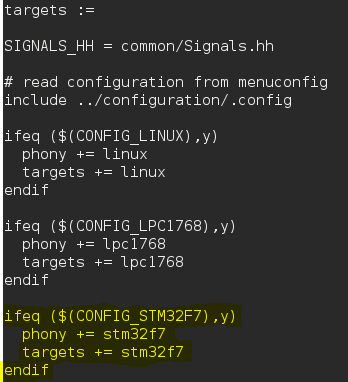
\includegraphics[width=9cm]{grafiken/Makefile_runtime1.png}
\end{center}
\end{figure}
\clearpage
\begin{figure}[h]
\begin{center}
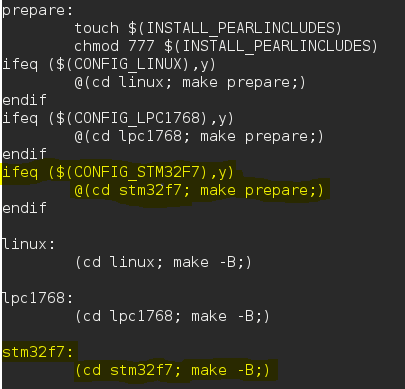
\includegraphics[width=11cm]{grafiken/Makefile_runtime2.png}
\end{center}
\end{figure}

\begin{figure}[h]
\begin{center}
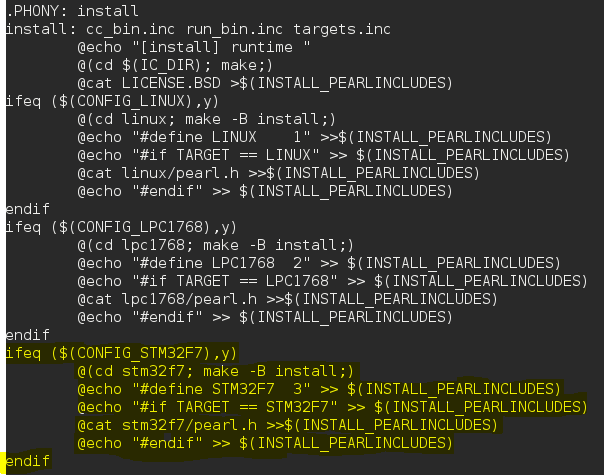
\includegraphics[width=15cm]{grafiken/Makefile_runtime3.png}
\end{center}
\end{figure}
\clearpage
\begin{figure}[h]
\begin{center}
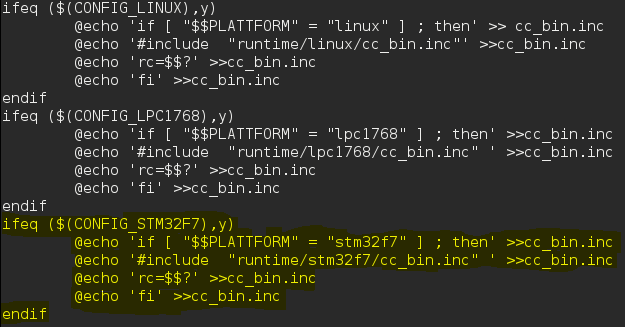
\includegraphics[width=16cm]{grafiken/Makefile_runtime4.png}
\end{center}
\end{figure}

\begin{figure}[h]
\begin{center}
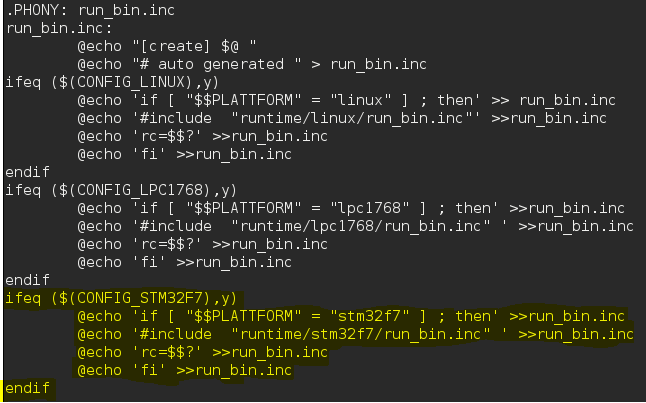
\includegraphics[width=16cm]{grafiken/Makefile_runtime5.png}
\end{center}
\end{figure}
\clearpage
\section{Änderungen der Makefile im Ordner stm32f7}\label{Änderungen der Makefile im Ordner stm32f7}
\begin{figure}[h]
\begin{center}
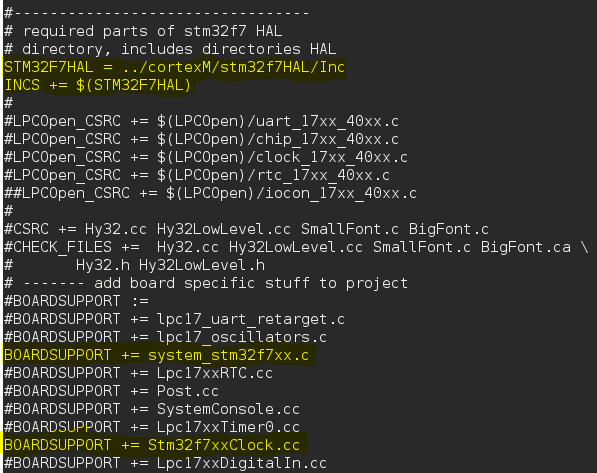
\includegraphics[width=13cm]{grafiken/Makefile_stm32f7_1.png}
\end{center}
\end{figure}

\begin{figure}[h]
\begin{center}
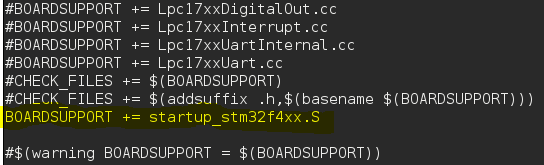
\includegraphics[width=13cm]{grafiken/Makefile_stm32f7_2.png}
\end{center}
\end{figure}
\newpage

\begin{figure}[h]
\begin{center}
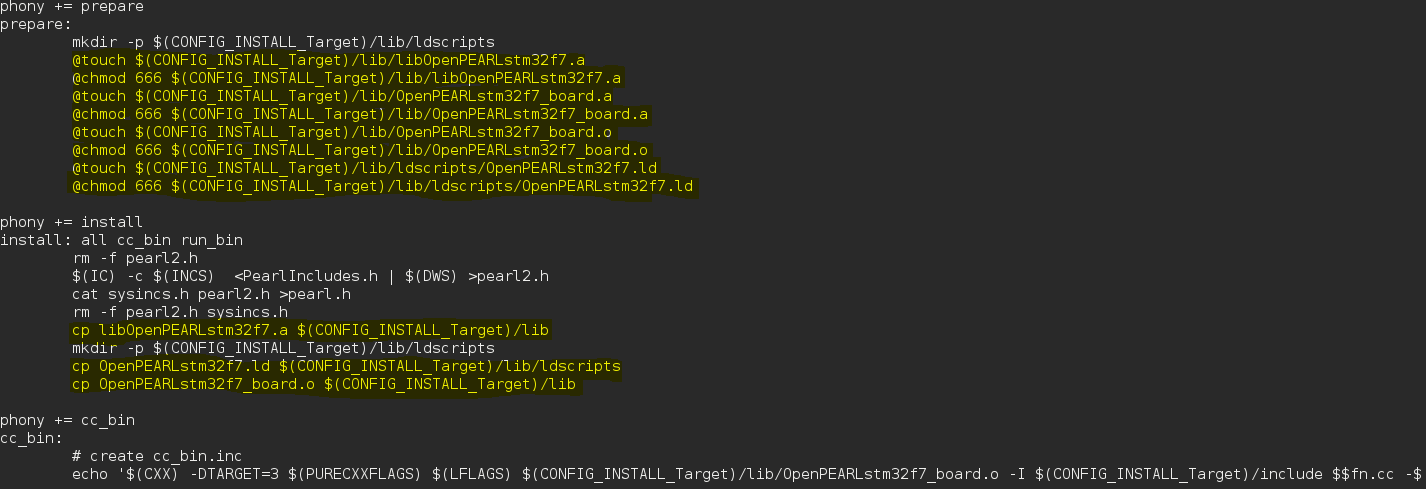
\includegraphics[width=35cm]{grafiken/Makefile_stm32f7_3.png}
\end{center}
\end{figure}


\end{document}